% =====================================================================
%  PROYECTO DE GRADO — Ingeniería de Sistemas, UMSS
%  Sistema Inteligente de Entrenamiento en Gimnasios con Realidad
%  Aumentada e Inteligencia Artificial
%
%  Compilar:  pdflatex main  ->  pdflatex main   (o: latexmk -pdf main.tex)
%  En Overleaf: subir la carpeta completa y compilar con pdfLaTeX.
% =====================================================================
\documentclass[11pt, letterpaper, oneside]{report}

% =====================================================================
%  PAQUETES Y FORMATO GENERAL
% =====================================================================

% =====================================================================
%  Formato según la "Guía para la elaboración de trabajos de grado"
%  (Carreras de Ing. Informática e Ing. de Sistemas, FCyT-UMSS, 2013):
%   - Fuente Arial 11 (párrafos), 12 MAYÚSCULAS (títulos), 11 (subtítulos)
%   - Interlineado sencillo, espaciado posterior 6 pt, justificado, sin sangría
%   - Carta; márgenes izq. 3 cm, der. 2 cm, sup. 2 cm, inf. 2 cm
%   - Número de página en el pie, centrado
%   - Figuras y cuadros: número, descripción y fuente DEBAJO; centrados y con recuadro
% =====================================================================

% ---------- Fuente Arial ----------
% Con XeLaTeX/LuaLaTeX se usa Arial real (o TeX Gyre Heros si no está instalada).
% Con pdfLaTeX se usa Helvetica, de métricas equivalentes a Arial.
\usepackage{iftex}
\ifPDFTeX
  \usepackage[utf8]{inputenc}
  \usepackage[T1]{fontenc}
  \usepackage[scaled=1]{helvet}
  \renewcommand{\familydefault}{\sfdefault}
\else
  \usepackage{fontspec}
  \IfFontExistsTF{Arial}{\setmainfont{Arial}\setsansfont{Arial}}
                       {\setmainfont{TeX Gyre Heros}\setsansfont{TeX Gyre Heros}}
\fi
\usepackage[spanish, es-tabla, es-noshorthands, es-nodecimaldot]{babel}
\usepackage{csquotes}

% ---------- Página carta y márgenes ----------
\usepackage[letterpaper, top=2cm, bottom=2cm, left=3cm, right=2cm,
            headheight=14pt, footskip=1cm]{geometry}

% ---------- Gráficos, colores y diagramas ----------
\usepackage{graphicx}
\usepackage[table]{xcolor}
\usepackage{tikz}
\usetikzlibrary{positioning, arrows.meta, shapes.geometric, shapes.misc,
                fit, backgrounds, calc, shadows, shapes.multipart}
\usepackage{pgfgantt}

% ---------- Tablas ----------
\usepackage{array}
\usepackage{booktabs}
\usepackage{tabularx}
\usepackage{longtable}
\usepackage{needspace}
\setlength{\LTpost}{2pt}
\usepackage{multirow}
\usepackage{makecell}
\renewcommand{\arraystretch}{1.25}
% Tablas con cuadrícula: bordes en todas las celdas y encabezado sombreado
\definecolor{encabezado}{gray}{0.88}
\setlength{\arrayrulewidth}{0.5pt}
\newcolumntype{L}[1]{>{\raggedright\arraybackslash}p{#1}}
\newcolumntype{C}[1]{>{\centering\arraybackslash}p{#1}}
\newcolumntype{Y}{>{\raggedright\arraybackslash}X}

% ---------- Listas y leyendas ----------
\usepackage{enumitem}
\setlist{itemsep=2pt, topsep=4pt, parsep=0pt}
% Leyendas DEBAJO de figuras y cuadros: "Figura 2-1. Descripción. Fuente: ..."
\usepackage[font=small, labelfont=bf, labelsep=period, justification=centering,
            figureposition=bottom, tableposition=bottom, skip=6pt]{caption}
% Recuadro de las figuras
\setlength{\fboxsep}{0pt}
\setlength{\fboxrule}{0.5pt}
\usepackage{float}
\usepackage{amsmath, amssymb}

% ---------- Código fuente ----------
\usepackage{listings}
\definecolor{codegreen}{rgb}{0,0.5,0.2}
\definecolor{codegray}{rgb}{0.5,0.5,0.5}
\definecolor{codepurple}{rgb}{0.58,0,0.82}
\definecolor{backcolour}{rgb}{0.96,0.97,0.96}

\lstdefinelanguage{TypeScript}{
  keywords={abstract, any, as, async, await, boolean, break, case, catch,
    class, const, continue, default, else, enum, export, extends, false,
    finally, for, from, function, if, implements, import, in, interface,
    let, new, null, number, of, private, public, readonly, return, string,
    switch, this, throw, true, try, type, typeof, undefined, void, while},
  sensitive=true,
  comment=[l]{//},
  morecomment=[s]{/*}{*/},
  morestring=[b]",
  morestring=[b]',
  morestring=[b]`
}

\lstdefinelanguage{FirestoreRules}{
  keywords={rules_version, service, match, allow, if, function, return,
    let, read, write, create, update, delete, true, false, is, in},
  sensitive=true,
  comment=[l]{//},
  morestring=[b]'
}

\lstdefinestyle{tesis}{
  backgroundcolor=\color{backcolour},
  commentstyle=\color{codegreen}\itshape,
  keywordstyle=\color{magenta!70!black}\bfseries,
  numberstyle=\tiny\color{codegray},
  stringstyle=\color{codepurple},
  basicstyle=\ttfamily\scriptsize,
  breakatwhitespace=false,
  breaklines=true,
  captionpos=b,
  keepspaces=true,
  numbers=left,
  numbersep=6pt,
  showspaces=false,
  showstringspaces=false,
  showtabs=false,
  tabsize=2,
  frame=single,
  rulecolor=\color{black!20},
  xleftmargin=1.5em,
  framexleftmargin=1.2em,
  extendedchars=true,
  literate=
    {á}{{\'a}}1 {é}{{\'e}}1 {í}{{\'i}}1 {ó}{{\'o}}1 {ú}{{\'u}}1
    {Á}{{\'A}}1 {É}{{\'E}}1 {Í}{{\'I}}1 {Ó}{{\'O}}1 {Ú}{{\'U}}1
    {ñ}{{\~n}}1 {Ñ}{{\~N}}1 {ü}{{\"u}}1 {¿}{{?`}}1 {¡}{{!`}}1
    {→}{{$\rightarrow$}}1 {·}{{$\cdot$}}1 {…}{{...}}3
    {—}{{--}}2 {─}{{-}}1 {│}{{|}}1 {├}{{+}}1 {└}{{+}}1 {┌}{{+}}1
    {┐}{{+}}1 {┘}{{+}}1 {┬}{{+}}1 {┴}{{+}}1 {┼}{{+}}1 {┤}{{+}}1
    {̀}{{\textbackslash{}u0300}}6 {ͯ}{{\textbackslash{}u036f}}6
}
\lstset{style=tesis}
\renewcommand{\lstlistingname}{Código}
\renewcommand{\lstlistlistingname}{ÍNDICE DE CÓDIGOS FUENTE}

% ---------- Hipervínculos ----------
\usepackage[hyphens]{url}
\usepackage{hyperref}
\hypersetup{
  colorlinks=true,
  linkcolor=black,
  urlcolor=black,
  citecolor=black,
  filecolor=black,
  pdftitle={Sistema inteligente de entrenamiento en gimnasios},
  pdfauthor={Erika Chino Alanoca}
}

% ---------- Bibliografía (estilo autor-año, compatible con APA) ----------
\usepackage[round, authoryear]{natbib}
\setcitestyle{aysep={,}}

% ---------- Interlineado y párrafos ----------
\usepackage{setspace}
\singlespacing                   % interlineado sencillo
\setlength{\parindent}{0pt}      % sin sangría
\setlength{\parskip}{6pt}        % espaciado posterior 6 pt

% ---------- Encabezados y pies de página ----------
\usepackage{fancyhdr}
\pagestyle{fancy}
\fancyhf{}
\fancyfoot[C]{\thepage}         % número de página centrado en el pie
\renewcommand{\headrulewidth}{0pt}
\fancypagestyle{plain}{\fancyhf{}\fancyfoot[C]{\thepage}\renewcommand{\headrulewidth}{0pt}}

% ---------- Numeración: capítulos en romanos, secciones en arábigos ----------
\renewcommand{\thechapter}{\Roman{chapter}}
\renewcommand{\thesection}{\arabic{chapter}.\arabic{section}}
\renewcommand{\thefigure}{\arabic{chapter}-\arabic{figure}}
\renewcommand{\thetable}{\arabic{chapter}-\arabic{table}}
\AtBeginDocument{\renewcommand{\thelstlisting}{\arabic{chapter}-\arabic{lstlisting}}}
\renewcommand{\theequation}{\arabic{chapter}.\arabic{equation}}
\setcounter{secnumdepth}{3}
\setcounter{tocdepth}{2}

% ---------- Títulos y subtítulos ----------
% Títulos (capítulos): 12 pt, negrilla, MAYÚSCULAS, centrados, 6 pt antes y después.
% Subtítulos: 11 pt, negrilla, alineados a la izquierda, 6 pt antes y después.
\usepackage{titlesec}
\newcommand{\fuentetitulo}{\fontsize{12}{14}\selectfont}
\titleformat{\chapter}[block]
  {\normalfont\fuentetitulo\bfseries\centering}
  {\MakeUppercase{\chaptertitlename}\ \thechapter:\ }
  {0pt}
  {\MakeUppercase}
\titlespacing*{\chapter}{0pt}{0pt}{6pt}
\titleformat{\section}{\normalfont\normalsize\bfseries}{\thesection.}{0.5em}{}
\titleformat{\subsection}{\normalfont\normalsize\bfseries}{\thesubsection.}{0.5em}{}
\titleformat{\subsubsection}{\normalfont\normalsize\bfseries}{\thesubsubsection.}{0.5em}{}
\titlespacing*{\section}{0pt}{6pt}{0pt}
\titlespacing*{\subsection}{0pt}{6pt}{0pt}
\titlespacing*{\subsubsection}{0pt}{6pt}{0pt}
\titlespacing*{\paragraph}{0pt}{6pt}{0.5em}

% ---------- Nombres en español ----------
\addto\captionsspanish{%
  \renewcommand{\contentsname}{ÍNDICE GENERAL}%
  \renewcommand{\listfigurename}{ÍNDICE DE FIGURAS}%
  \renewcommand{\listtablename}{ÍNDICE DE TABLAS}%
  \renewcommand{\appendixname}{Anexo}%
  \renewcommand{\chaptername}{Capítulo}%
}
% En los anexos la etiqueta es "ANEXO A -- ..."
\usepackage{etoolbox}
\appto\appendix{%
  \renewcommand{\thechapter}{\Alph{chapter}}%
  \renewcommand{\thesection}{\Alph{chapter}.\arabic{section}}%
  \renewcommand{\thefigure}{\Alph{chapter}-\arabic{figure}}%
  \renewcommand{\thetable}{\Alph{chapter}-\arabic{table}}%
  \renewcommand{\thelstlisting}{\Alph{chapter}.\arabic{lstlisting}}%
}

% ---------- Ancho de números en los índices ----------
\usepackage{tocloft}
\renewcommand{\cftchapfont}{\bfseries}
\renewcommand{\cftchappagefont}{\bfseries}
\setlength{\cftchapnumwidth}{2.6em}
\setlength{\cftsecnumwidth}{2.6em}
\setlength{\cftsubsecnumwidth}{3.4em}
\setlength{\cftfignumwidth}{2.8em}
\setlength{\cfttabnumwidth}{2.8em}
% Títulos de los índices: 12 pt, negrilla, centrados, sin salto de página propio
\renewcommand{\cfttoctitlefont}{\hfill\fuentetitulo\bfseries}
\renewcommand{\cftaftertoctitle}{\hfill}
\renewcommand{\cftloftitlefont}{\hfill\fuentetitulo\bfseries}
\renewcommand{\cftafterloftitle}{\hfill}
\renewcommand{\cftlottitlefont}{\hfill\fuentetitulo\bfseries}
\renewcommand{\cftafterlottitle}{\hfill}
\setlength{\cftbeforetoctitleskip}{0pt}
\setlength{\cftaftertoctitleskip}{6pt}
\setlength{\cftbeforeloftitleskip}{12pt}
\setlength{\cftafterloftitleskip}{6pt}
\setlength{\cftbeforelottitleskip}{12pt}
\setlength{\cftafterlottitleskip}{6pt}
\setlength{\cftbeforechapskip}{4pt}
\setlength{\emergencystretch}{2em}

% =====================================================================
%  VARIABLES GLOBALES DEL PROYECTO DE GRADO
%  (cambiar aquí y se actualiza en todo el documento)
% =====================================================================

% Datos institucionales
\newcommand{\universidad}{UNIVERSIDAD MAYOR DE SAN SIMÓN}
\newcommand{\facultad}{FACULTAD DE CIENCIAS Y TECNOLOGÍA}
\newcommand{\carrera}{CARRERA DE INGENIERÍA DE SISTEMAS}
\newcommand{\ubicacion}{Cochabamba -- Bolivia}
\newcommand{\fechaDefensa}{2026}  % TODO: mes-año de la defensa, p. ej. 11-2026

% Datos del proyecto
\newcommand{\tituloTesis}{SISTEMA INTELIGENTE DE ENTRENAMIENTO EN GIMNASIOS CON REALIDAD AUMENTADA E INTELIGENCIA ARTIFICIAL}
\newcommand{\modalidadTesis}{Proyecto de Grado presentado para optar al Diploma Académico de Licenciatura en Ingeniería de Sistemas}
\newcommand{\nombreApp}{CoachApp}

% Personas
\newcommand{\autorTesis}{Erika Chino Alanoca}
\newcommand{\tutorTesis}{Mgr. Jimmy Villarroel Novillo}
\newcommand{\docenteTesis}{MSc. Américo Fiorilo Lozada}

% =====================================================================
%  COMANDOS PROPIOS
% =====================================================================

% Nombre de archivo, ruta o identificador de código dentro del texto
\newcommand{\archivo}[1]{\texttt{\small #1}}

% Marca visible para lo que la autora debe completar antes de imprimir.
% Para ocultar todas las marcas: \renewcommand{\pendiente}[1]{}
\newcommand{\pendiente}[1]{\textcolor{red!70!black}{\textbf{[PENDIENTE:} #1\textbf{]}}}

% Captura de pantalla de la app.
%   \captura{archivo-sin-extension}{Leyenda}{etiqueta}
% Coloca las capturas en figuras/capturas/ (png o jpg). Mientras el archivo
% no exista, se dibuja un recuadro con el nombre esperado.
\newcommand{\captura}[3]{%
  \begin{figure}[H]
    \centering
    \IfFileExists{figuras/capturas/#1.png}{%
      \includegraphics[height=0.42\textheight]{figuras/capturas/#1.png}}{%
    \IfFileExists{figuras/capturas/#1.jpg}{%
      \includegraphics[height=0.42\textheight]{figuras/capturas/#1.jpg}}{%
      \fbox{\parbox[c][0.30\textheight][c]{0.32\textwidth}{\centering\small
        Captura de pantalla\\[4pt]\texttt{\scriptsize figuras/capturas/}\\\texttt{\scriptsize\detokenize{#1}.png}}}}}
    \caption{#2}
    \label{#3}
  \end{figure}}

% Dos capturas lado a lado
%   \capturados{archivo1}{subleyenda1}{archivo2}{subleyenda2}{Leyenda}{etiqueta}
\newcommand{\imagencaptura}[1]{%
  \IfFileExists{figuras/capturas/#1.png}{%
    \includegraphics[height=0.36\textheight]{figuras/capturas/#1.png}}{%
  \IfFileExists{figuras/capturas/#1.jpg}{%
    \includegraphics[height=0.36\textheight]{figuras/capturas/#1.jpg}}{%
    \fbox{\parbox[c][0.28\textheight][c]{0.44\textwidth}{\centering\small
      Captura de pantalla\\[4pt]\texttt{\scriptsize figuras/capturas/}\\\texttt{\scriptsize\detokenize{#1}.png}}}}}}
\newcommand{\capturados}[6]{%
  \begin{figure}[H]
    \centering
    \begin{minipage}[t]{0.47\textwidth}\centering
      \imagencaptura{#1}\\[2pt]{\small (a) #2}
    \end{minipage}\hfill
    \begin{minipage}[t]{0.47\textwidth}\centering
      \imagencaptura{#3}\\[2pt]{\small (b) #4}
    \end{minipage}
    \caption{#5}
    \label{#6}
  \end{figure}}

% Nota de fuente al pie de tablas y figuras
\newcommand{\fuente}[1]{\par\vspace{2pt}{\footnotesize\textit{Fuente:} #1}}

% Estilos TikZ comunes para diagramas
\tikzset{
  caja/.style={rectangle, rounded corners=3pt, draw=black!70, fill=white,
               minimum height=0.9cm, align=center, font=\small, inner sep=5pt},
  capa/.style={rectangle, draw=black!60, fill=#1, minimum width=13.5cm,
               minimum height=1.6cm, align=left, font=\small},
  capa/.default={black!5},
  flecha/.style={-{Stealth[length=2.5mm]}, thick, black!70},
  flechad/.style={-{Stealth[length=2.5mm]}, thick, dashed, black!60},
  casouso/.style={ellipse, draw=black!70, fill=green!4, minimum width=3.6cm,
                  minimum height=0.85cm, align=center, font=\footnotesize, inner sep=1pt},
  entidad/.style={rectangle, draw=black!70, fill=white, align=left,
                  font=\scriptsize\ttfamily, inner sep=4pt, rectangle split,
                  rectangle split parts=2, rectangle split part fill={green!12,white}},
}

% Actor UML (monigote) — \actor{nombre-nodo}{posición}{etiqueta}
\newcommand{\actor}[3]{%
  \begin{scope}[shift={#2}]
    \draw[thick] (0,0.55) circle (0.18);
    \draw[thick] (0,0.37) -- (0,-0.15);
    \draw[thick] (-0.3,0.2) -- (0.3,0.2);
    \draw[thick] (0,-0.15) -- (-0.25,-0.55);
    \draw[thick] (0,-0.15) -- (0.25,-0.55);
    \node[font=\small, below] at (0,-0.6) {#3};
    \coordinate (#1) at (0.35,0.1);
  \end{scope}}

% Lista con viñetas dentro de una celda de tabla (columnas p{} / X)
\newenvironment{tablista}
  {\begin{itemize}[leftmargin=1.1em, nosep, topsep=0pt, partopsep=0pt,
     before={\vspace{-0.55\baselineskip}}, after={\vspace{-\baselineskip}}]}
  {\end{itemize}}

% Párrafo de "Conclusión:" debajo de las tablas comparativas
\newcommand{\conclusion}[1]{\par\textbf{Conclusión:} #1\par}

% Encabezado en negrita dentro de una sección (sin numerar)
\newcommand{\titulillo}[1]{\par\medskip\noindent\textbf{#1}\par}

% Lista de referencias con sangría francesa (formato APA)
\newenvironment{referenciasapa}
  {\begin{list}{}{\setlength{\leftmargin}{1.27cm}\setlength{\itemindent}{-1.27cm}
     \setlength{\itemsep}{6pt}\setlength{\parsep}{0pt}}\raggedright}
  {\end{list}}


\begin{document}

% ---------------- Páginas preliminares ----------------
\begin{titlepage}
    \centering

    % Encabezado con los dos logos
    \begin{minipage}[c]{0.18\textwidth}
        
\includegraphics[width=\textwidth]{figuras/logo_umss.png}
    \end{minipage}%
    \begin{minipage}[c]{0.64\textwidth}
        \centering
        {\bfseries \small \universidad \par}
        \vspace{0.1cm}
        {\bfseries \small \facultad \par}
        \vspace{0.1cm}
        {\bfseries \small \carrera \par}
    \end{minipage}%
    \begin{minipage}[c]{0.18\textwidth}
        
\includegraphics[width=\textwidth]{figuras/logo_fcyt.jpg}
    \end{minipage}

    \vspace{3cm}

    % Cuadro del título
    \setlength{\fboxrule}{1.5pt}
    \setlength{\fboxsep}{14pt}
    \fbox{%
        \begin{minipage}{0.85\textwidth}
            \centering
            \bfseries \large \tituloTesis
        \end{minipage}%
    }

    \vspace{2.5cm}

    \begin{minipage}{0.8\textwidth}
        \centering
        \small \modalidadTesis
    \end{minipage}

    \vspace{3cm}

    % Datos de la autora, tutor y docente
    \begin{raggedright}
        \hspace{0.05\textwidth}
        \begin{tabular}{ll}
            \textbf{Presentado por:} & \autorTesis \\[0.2cm]
            \textbf{Tutor:}          & \tutorTesis
        \end{tabular}
    \end{raggedright}

    \vfill

    {\bfseries \small \ubicacion \par}
    \vspace{0.1cm}
    {\bfseries \small \fechaDefensa \par}
\end{titlepage}


\pagenumbering{roman}
\clearpage
\thispagestyle{plain}

\begin{center}
    {\Large \bfseries AGRADECIMIENTOS}
\end{center}

\vspace{0.8cm}

% TODO: escribir los agradecimientos (en el documento Word esta página
% estaba vacía).
\pendiente{Escribir los agradecimientos.}

\vfill

\clearpage
\thispagestyle{plain}

\begin{center}
    {\Large \bfseries FICHA RESUMEN}
\end{center}

\vspace{0.3cm}

\begin{tabular}{@{}ll}
\textbf{Grado:} & Licenciatura en Ingeniería de Sistemas \\
\textbf{Modalidad:} & Proyecto de Grado \\
\textbf{Facultad:} & Ciencias y Tecnología \\
\textbf{Carrera:} & Ingeniería de Sistemas \\
\textbf{Título del trabajo:} & \parbox[t]{10cm}{Sistema Inteligente de Entrenamiento en
Gimnasios con Realidad Aumentada e Inteligencia Artificial} \\
\textbf{Autora:} & \autorTesis \\
\textbf{Tutor:} & \tutorTesis \\
\end{tabular}

\vspace{0.4cm}

En el primer capítulo se realizó una investigación sobre los antecedentes y se
analizó la problemática relacionada con el abandono temprano de los usuarios de
gimnasios, atribuida principalmente a la falta de orientación, motivación y
seguimiento personalizado. A partir de ello, se propone el diseño de un sistema
inteligente capaz de guiar al usuario en uso correcto de máquinas, personalizar
rutinas de entrenamiento y registrar su progreso físico.

En el segundo capítulo se desarrolla el marco teórico que sustenta la solución
tecnológica. Se revisan distintas metodologías de desarrollo de software,
comparando enfoques tradicionales y ágiles, y se justifica la selección de
Mobile-D como la metodología más adecuada para este proyecto.

En el tercer capítulo se detalla el área de aplicación y se describe la
adopción de la metodología Mobile-D en el desarrollo del sistema, especificando
su aplicación práctica en fases de exploración, inicialización, producción,
estabilización y pruebas.


% Índice de contenido, de cuadros y de figuras en una sola hoja (guía, punto 4)
\clearpage
\tableofcontents
\listoftables
\listoffigures
\clearpage

% ---------------- Cuerpo ----------------
\pagenumbering{arabic}

\chapter{INTRODUCCIÓN}
\label{cap:introduccion}

En la actualidad, la práctica del ejercicio físico en gimnasios ha cobrado gran
relevancia como parte de un estilo de vida saludable. Sin embargo, diversos
estudios han evidenciado que una gran parte de los usuarios abandonan sus
rutinas en los primeros meses, principalmente por la falta de orientación,
motivación y seguimiento personalizado (Gjestvang, 2020). Esta problemática
afecta especialmente a los principiantes, quienes enfrentan barreras como el
desconocimiento del uso correcto de las máquinas, el alto coste de entrenadores
personales y la ausencia de planificación estructurada.

En respuesta a esta necesidad, se han desarrollado diversas soluciones
tecnológicas que buscan mejorar la experiencia del usuario en el gimnasio, como
aplicaciones móviles con realidad aumentada (Cruz, 2024) y sistemas de
información para rutinas y dietas (Fernández, 2018). No obstante, muchas de
estas herramientas carecen de personalización profunda y seguimiento
inteligente.

Este proyecto propone el desarrollo de una aplicación móvil basada en realidad
aumentada e inteligencia artificial, orientada a guiar a los usuarios en el uso
correcto de máquinas de ejercicio, planificar rutinas personalizadas y realizar
un seguimiento del progreso físico. La solución busca democratizar el acceso a
la orientación profesional, reducir el abandono temprano y fomentar la
constancia en el entrenamiento físico, utilizando tecnologías modernas como
React Native, Firebase y TensorFlow Lite.

Con esto, se pretende contribuir no solo al bienestar individual, sino también
a la optimización de recursos en gimnasios, ofreciendo una herramienta
accesible, interactiva y eficaz para la autogestión del entrenamiento.

% =====================================================================
\section{Antecedentes}
\label{sec:antecedentes}

(Yépez, 2017) en su proyecto de grado cuyo objetivo principal es la creación de
un gimnasio que combine asesoramiento presencial y virtual, orientado a la nueva
disciplina llamada Street Workout, que consiste en utilizar el propio peso
corporal para ejercitarse.

(Gjestvang, 2020) se realizó un estudio longitudinal en Noruega con el objetivo
de identificar las principales barreras en la iniciación y adherencia al
ejercicio en gimnasios. El proyecto evidenció que entre el 40\,\% y el 65\,\% de
los nuevos usuarios abandonan la asistencia regular en los primeros meses,
principalmente por la falta de motivación, orientación adecuada y seguimiento
personalizado. Estos resultados destacan la importancia de diseñar
herramientas tecnológicas que fortalezcan la adherencia a programas de
ejercicio estructurados.

(Cruz, 2024) desarrolló un proyecto de grado desarrollado en la Universidad
Mayor de San Simón, una aplicación móvil para gimnasios que utiliza escaneo de
código QR con realidad aumentada para mejorar la experiencia de los usuarios y
la gestión de entrenamientos, que permite a los usuarios obtener instrucciones
detalladas en tiempo real sobre los ejercicios.

(Fernandez, 2018) en su proyecto de grado desarrolló un sistema de información
cuyo objetivo principal es brindar apoyo a los usuarios o clientes de los
gimnasios, proporcionándoles rutinas de ejercicios y dietas, para que sirva de
guía sobre cómo usar las máquinas y como administrar sus alimentos para obtener
el objetivo deseado.

(BodBot IA Entrenador Personal, 2016) es una plataforma de fitness avanzada
creada por Edward Laux, Jason Storm y Sergio Prado, que ofrece entrenamientos de
IA personalizados según los objetivos, equipos, capacidades físicas y
dificultad del usuario, esta plataforma proporciona una guía paso a paso para
cada ejercicio, contiene personalización de peso corporal y registro de
alimentación diario.

(Ejercicios en el Gimnasio, 2021) desarrollada por Leap Fitness Group, es una
plataforma fitness para principiantes y asiduos al gimnasio, que funciona como
un entrenador personalizado, creando rutinas, mostrando la postura correcta para
realizar ejercicios esto por medio de instrucciones visuales y literales
explícitas, siguiendo el progreso con estadísticas y gráficos claros.

% =====================================================================
\section{Análisis del problema}
\label{sec:problema}

\subsection{Descripción del problema}

Este proyecto surge para resolver las principales barreras que los usuarios de
gimnasios enfrentan, particularmente la falta de orientación adecuada y la falta
de estructura en sus entrenamientos. (Gjestvang, 2020) Estudios demuestran que
entre el 40\,\% y el 65\,\% de los nuevos usuarios abandonan el gimnasio en los
primeros meses, principalmente por la falta de guía y seguimiento
personalizado. Los principales problemas identificados incluyen:

\begin{itemize}
    \item \textbf{Falta de conocimiento sobre el uso adecuado de las máquinas y
    la postura correcta:} Esto lleva a errores que pueden causar lesiones y
    dificultar el progreso hacia los objetivos físicos.
    \item \textbf{Costo elevado de los entrenadores personales:} Muchas personas
    no pueden acceder a una guía profesional debido al costo asociado, lo cual
    deja a la mayoría sin un apoyo adecuado.
    \item \textbf{Falta de seguimiento del progreso:} La falta de un sistema para
    registrar y analizar el progreso personal desmotiva a los usuarios, ya que
    no tienen una forma clara de visualizar sus avances.
    \item \textbf{Carencia de planificación estructurada del entrenamiento:} Sin
    una rutina clara y bien planificada, muchos usuarios se sienten perdidos y no
    logran aprovechar el tiempo de entrenamiento, lo cual fomenta la
    desmotivación y el abandono.
\end{itemize}

\subsection{Definición del problema}

¿Cómo desarrollar una aplicación para gimnasios que ofrezca seguimiento rutinas
de ejercicio personalizadas con Inteligencia artificial?

% =====================================================================
\section{Objetivos}
\label{sec:objetivos}

\subsection{Objetivo general}

Desarrollar un sistema inteligente para el entrenamiento en gimnasios,
proporcionando una guía estructurada y seguimiento personalizado de los
ejercicios.

\subsection{Objetivos específicos}

\begin{itemize}
    \item Guiar sobre el uso correcto de máquinas.
    \item Instruir en la ejecución correcta de ejercicios específicos.
    \item Diseñar rutinas de entrenamiento personalizadas y estructuradas,
    adaptadas a los objetivos de cada usuario.
    \item Construir herramientas de planificación que permitan a los usuarios
    organizar sus entrenamientos de manera eficiente.
    \item Registrar la ingesta de alimentos con el fin de controlar y evaluar las
    calorías consumidas por el usuario.
    \item Implementar un sistema de seguimiento del progreso físico.
    \item Generar reportes personalizados de progreso físico.
\end{itemize}

% =====================================================================
\section{Área de conocimiento}
\label{sec:area}

\textbf{Área:} Programación Móvil

\textbf{Subárea:} Sistema de Información

% =====================================================================
\section{Alcance}
\label{sec:alcance}

\begin{itemize}
    \item El sistema funcionará en sistemas operativos Android.
    \item Interfaz intuitiva para el registro de usuarios.
    \item Guía sobre el uso correcto de máquinas de gimnasio.
    \item Registrar el progreso físico (peso, estatura, edad, masa corporal).
    \item Creación de rutinas personalizadas según los objetivos del usuario.
    \item El registro de alimentación se limitará solo al conteo calórico, es
    decir una calculadora de IMC.
    \item El sistema no reemplaza la supervisión profesional de entrenadores o
    nutricionistas.
    \item No se contempla la integración con dispositivos externos (smartwatch,
    banda de frecuencia cardíaca, entre otros).
\end{itemize}

% =====================================================================
\section{Justificación}
\label{sec:justificacion}

\subsection{Justificación técnica}

El proyecto es técnicamente viable gracias a la combinación de tecnologías
modernas y flexibles. Se empleará React Native con Expo para garantizar una
experiencia fluida en dispositivos Android, permitiendo un desarrollo
multiplataforma con una sola base de código.

La base de datos y autenticación estarán gestionadas por Firebase, lo que
asegura escalabilidad, sincronización en tiempo real y seguridad en el manejo de
datos de usuarios.

El componente de inteligencia artificial se implementará para generar rutinas
personalizadas, basándose en parámetros como peso, altura, edad, nivel de
experiencia y objetivos físicos. Este módulo podrá entrenarse mediante modelos
preexistentes o redes neuronales ligeras optimizadas para dispositivos móviles.

Además, se integrará un sistema de visualización interactiva con imágenes o
animaciones que muestran la postura correcta en cada ejercicio, lo cual aumenta
la comprensión y reduce el riesgo de lesiones.

En conjunto, estas tecnologías garantizan un sistema robusto, escalable y con
potencial de expansión futura.

\subsection{Justificación económica}

La aplicación representa una alternativa de bajo costo frente a los servicios
tradicionales de entrenamiento personalizado. Al automatizar la generación de
rutinas mediante inteligencia artificial, se reducen los costos asociados a la
contratación de entrenadores físicos, permitiendo que los usuarios obtengan
orientación profesional sin incurrir en gastos adicionales.

Para los gimnasios, la herramienta puede convertirse en un complemento
estratégico que optimice el tiempo de los entrenadores y mejore la retención de
clientes, al ofrecerles una plataforma moderna de autogestión del
entrenamiento. Asimismo, el desarrollo de esta aplicación se apoya en
tecnologías de código abierto (React Native, Firebase, TensorFlow Lite, etc.),
lo que disminuye considerablemente los costos de desarrollo y mantenimiento del
sistema.

\subsection{Justificación social}

Este proyecto busca eliminar las barreras que limitan la práctica constante del
ejercicio físico, ofreciendo orientación y motivación a través de la tecnología.
Está dirigido principalmente a usuarios principiantes o personas que no tienen
acceso a un entrenador personal. Contribuye a la promoción de un estilo de vida
saludable, fomenta la constancia y previene lesiones al enseñar el uso correcto
de las máquinas.

\chapter{MARCO TEÓRICO}
\label{cap:marco}

% =====================================================================
\section{Metodología de Desarrollo}
\label{sec:metodologia-desarrollo}

Una metodología de desarrollo de software es un marco de trabajo que se usa
para estructurar, planificar y controlar el proceso de desarrollo de sistemas de
información (Gabriel Maide \& Pacienzia, 2020). Asimismo el objetivo de las
distintas metodologías es el intentar organizar los equipos de trabajo para que
estos desarrollen las funciones de un programa de la mejor manera posible
(Santander, 2020). Una metodología establece un conjunto de prácticas, técnicas
y procesos que permiten mejorar la eficiencia del trabajo, garantizar la
calidad y reducir la incertidumbre durante el ciclo de vida del software
(Pressman, 2010).

Las metodologías de desarrollo proporcionan lineamientos que facilitan la
coordinación del equipo, la definición clara de los requerimientos, la gestión
de riesgos y la evaluación del avance del proyecto. El uso de la metodología
adecuada contribuye a la minimización de riesgos, estandarización de
procedimientos y mejorar la productividad.

Las metodologías de desarrollo de software son enfoques que proporcionan un
marco claro para planificar, ejecutar y entregar proyectos de software, estas
pueden ser lineales o iterativas, se ajustan a diferentes tipos de proyectos y
equipos de acuerdo a las necesidades específicas de cada proyecto o equipo
(Team, 2024).

% =====================================================================
\section{Metodologías de desarrollo de software tradicionales vs ágiles}
\label{sec:tradicionales-agiles}

Las metodologías de desarrollo de software se agrupan principalmente en
tradicionales y ágiles, cada una con enfoques y características distintas.

\subsection{Metodologías tradicionales}

Las metodologías tradicionales, conocidas también como predictivas, son
enfoques secuenciales y lineales, basados en una planificación detallada y
estructurada, donde cada fase debe completarse antes de iniciar la siguiente,
tampoco se puede volver hacia atrás una vez se ha cambiado de fase. Estas
metodologías, no se adaptan nada bien a los cambios, y el mundo actual cambia
constantemente (Santander, 2020).

Este enfoque es ideal para proyectos en los que los requerimientos están bien
definidos desde el principio.

{\small
\begin{longtable}{L{2.6cm} L{6.8cm} L{5.4cm}}
\caption{Comparación de Metodologías tradicionales de desarrollo de software}
\label{tab:metodologias-tradicionales}\\
\toprule
\textbf{Metodología} & \textbf{Descripción} & \textbf{Características} \\
\midrule
\endfirsthead
\toprule
\textbf{Metodología} & \textbf{Descripción} & \textbf{Características} \\
\midrule
\endhead
\bottomrule
\endfoot
\textbf{Waterfall} & La metodología waterfall o cascada, es un proceso
secuencial, el proyecto se divide en fases, las cuales deben completarse
completamente antes de pasar a la siguiente. El avance del progreso va de
arriba hacia abajo. &
\begin{tablista}
  \item Enfoque lineal y estructurado.
  \item Requiere una planificación previa.
  \item No permite adaptaciones una vez iniciada la ejecución.
  \item Fácil de entender.
\end{tablista} \\
\midrule
\textbf{Espiral} & Esta metodología integra la gestión de riesgos a lo largo
del proceso de desarrollo. El desarrollo ocurre en ciclos o vueltas y cada uno
de estos cuenta con 4 fases: planificación, análisis de riesgos, ingeniería y
evaluación por parte del cliente. &
\begin{tablista}
  \item Enfoque iterativo basado en ciclos sucesivos.
  \item Permite incorporar ajustes o mejoras en cada iteración.
  \item Contempla análisis de riesgos periódico.
\end{tablista} \\
\midrule
\textbf{Incremental} & Esta metodología combina elementos de la metodología
cascada, permite desarrollar el producto de forma progresiva, cada etapa
incremental constituye una nueva funcionalidad, lo que permite ver resultados
de forma más rápida en comparación del modelo cascada. &
\begin{tablista}
  \item Entrega parcial del sistema.
  \item Facilita la detección de errores temprana.
  \item Recopila comentarios de clientes después de cada entrega.
  \item Flexible a los cambios.
  \item Combinación de enfoques lineales e iterativos.
\end{tablista} \\
\midrule
\textbf{Prototipado} & Esta metodología desarrolla un modelo preliminar y
tangible de software, esto permite que el usuario pruebe y de
retroalimentación, para así poder ajustar los requisitos y mejorar el diseño
del sistema final. &
\begin{tablista}
  \item Facilita la comunicación con el usuario.
  \item Reduce la incertidumbre.
  \item Es iterativa.
  \item Reduce riesgos y costos.
  \item Es flexible y versátil.
\end{tablista} \\
\midrule
\textbf{Diseño rápido de aplicaciones RAD} & Esta metodología permite
desarrollar software de alta calidad en un corto periodo de tiempo. Los costes
son mucho más altos y el desarrollo es flexible, aunque requiere mayor
intervención de los usuarios. &
\begin{tablista}
  \item Desarrollo basado en prototipos funcionales.
  \item Iteraciones cortas y desarrollo incremental.
  \item Alta participación del usuario.
\end{tablista} \\
\end{longtable}
}
\fuente{Elaboración propia.}

\conclusion{De acuerdo al análisis comparativo presentado en la
Tabla~\ref{tab:metodologias-tradicionales}, se concluye que la principal
diferencia entre las metodologías tradicionales radica en su tolerancia al
cambio y la gestión de riesgo. Mientras que el modelo cascada prioriza una
estructura secuencial y rígida, los modelos espiral, incremental y prototipado
introducen cambios iterativos que permiten la validación progresiva del
usuario. Por lo tanto, estas metodologías son más aptas para proyectos con
requerimientos claros, estables que no cambiaran con el tiempo.}

\subsection{Metodologías ágiles para móvil}

Las metodologías ágiles aplicadas al desarrollo móvil surgen como respuesta a
la necesidad de adaptarse a un entorno cambiante y a ciclos de producción
rápidos. Estas metodologías están centradas en la entrega continua de valor, la
colaboración constante con el cliente y la capacidad de adaptarse a nuevos
requerimientos.

Las metodologías ágiles son las más utilizadas en la actualidad debido a su alta
flexibilidad y agilidad (Santander, 2020). Se basan en la metodología
incremental, en la que en cada ciclo de desarrollo se agregan nuevas
funcionalidades a la aplicación final.

{\small
\begin{longtable}{L{2.4cm} L{7.2cm} L{5.2cm}}
\caption{Comparación de metodologías ágiles móviles}
\label{tab:metodologias-agiles}\\
\toprule
\textbf{Metodología} & \textbf{Descripción} & \textbf{Características} \\
\midrule
\endfirsthead
\toprule
\textbf{Metodología} & \textbf{Descripción} & \textbf{Características} \\
\midrule
\endhead
\bottomrule
\endfoot
\textbf{Scrum} & Es una metodología ágil, que divide los requerimientos y
tareas de forma similar a Kanban. Está compuesto por iteraciones fijas y cortas
denominadas Sprints, así como una estructura basada en roles, eventos y
artefactos definidos. Su objetivo es entregar incrementos funcionales del
producto en ciclos de 2 a 4 semanas, fomentando la colaboración y la
inspección continua (Schwaber \& Sutherland, 2020). &
\begin{tablista}
  \item Roles definidos (Product Owner, Scrum Master, Equipo).
  \item Iteraciones cortas y fijas.
  \item Entregas incrementales al final de cada sprint.
  \item Alta colaboración con el cliente.
  \item Uso de backlog y tableros para la gestión visual del trabajo.
  \item[] (Schwaber \& Sutherland, 2020)
\end{tablista} \\
\midrule
\textbf{Extreme Programming (XP)} & Es una metodología basada en relaciones
interpersonales, la colaboración y la retroalimentación continua. Su objetivo
principal es crear un entorno de trabajo basado en la comunicación constante,
simplicidad del diseño y participación activa del cliente. Incorpora prácticas
de ingeniería como pair programming, test-driven development, refactorización
constante e integración continua (Beck \& Andres, 2005). &
\begin{tablista}
  \item Trabajo colaborativo.
  \item Diseño sencillo y adaptables.
  \item Desarrollo guiado por pruebas.
  \item Refactorización continua.
  \item Integración continua.
  \item Entregas frecuentes y pequeñas iteraciones.
  \item Planificación basada en historias de usuario.
  \item Programación en parejas.
\end{tablista} \\
\midrule
\textbf{Mobile-D} & Es una metodología ágil para el desarrollo de aplicaciones
móviles para equipos pequeños, está centrada en ciclos de desarrollo rápidos y
entrega continua. Combina prácticas ágiles con procesos orientados al hardware
y ciclos muy cortos de entrega (Abrahamsson, y otros, 2004). &
\begin{tablista}
  \item Diseñada para desarrollo móvil.
  \item Iteraciones rápidas.
  \item Adaptación a restricciones de hardware.
  \item Enfocado en grupos pequeños.
\end{tablista} \\
\midrule
\textbf{Kanban} & Es una metodología de trabajo inventada por la empresa de
automóviles Toyota. Consiste en dividir las tareas en porciones mínimas y
organizarlas en un tablero de trabajo dividido en tareas pendientes, en curso y
finalizadas. De esta forma se crea un flujo de trabajo muy visual basado en
tareas prioritarias e incrementando el valor del producto (Santander, 2020). &
\begin{tablista}
  \item Visualización del trabajo.
  \item Límite de trabajo en curso.
  \item Mejora continua.
  \item No requiere iteraciones fijas.
  \item Fácil implementación en equipos individuales.
  \item Gestión visual del trabajo.
\end{tablista} \\
\end{longtable}
}
\fuente{Elaboración propia a partir de (Schwaber \& Sutherland, 2020); (Beck \&
Andres, 2005); (Santander, 2020); (Abrahamsson, y otros, 2004).}

\conclusion{En conclusión, todas las metodologías ágiles comparten principios
como la flexibilidad y la entrega continua, sin embargo, la metodología
Mobile-D es la más adecuada para proyectos móviles por su rapidez, sus
iteraciones cortas y su adaptación a las particularidades del hardware.}

% =====================================================================
\section{Mobile-D}
\label{sec:mobile-d}

La metodología Mobile-D es un enfoque ágil diseñado para el desarrollo de
software en dispositivos móviles. Surgió como resultado de investigaciones
realizadas por el VTT, con el objetivo de responder a los desafíos propios del
entorno móvil, como ciclos de producción acelerados, restricciones de hardware,
diversidad de plataformas y cambios frecuentes en los requisitos (Abrahamsson
et al., 2004).

Mobile-D es adecuada para proyectos que requieren rapidez, flexibilidad y alta
calidad, como aplicaciones de seguridad informática, plataformas de comercio
electrónico, aplicaciones de simulación entre otros. Está pensada para equipos
pequeños. Esta metodología combina prácticas de diversas metodologías ágiles,
como Scrum, XP y prácticas de ingeniería de software.

\subsection{Fases y etapas}

El desarrollo mediante el enfoque de Mobile-D se compone de 5 fases como se
muestra en la Figura~\ref{fig:mobile-d}, estas fases son: Exploración,
Inicialización, Producción, Estabilización y Pruebas del sistema.

\begin{figure}[H]
    \centering
    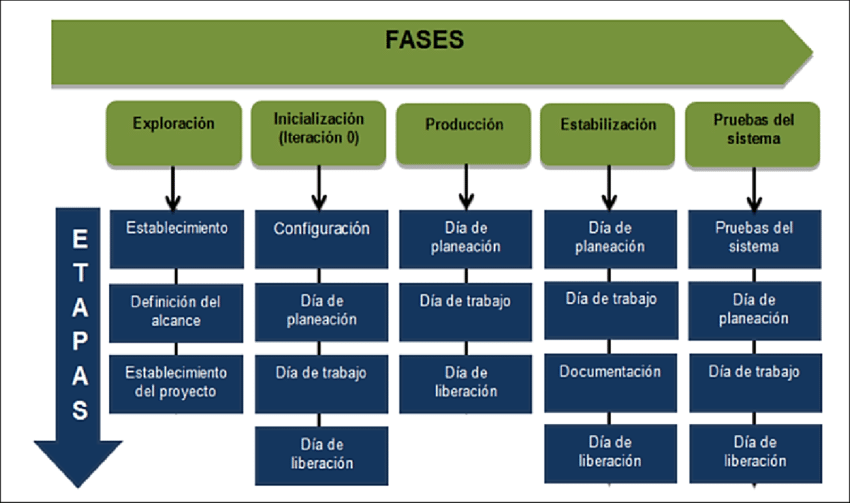
\includegraphics[width=0.85\textwidth]{figuras/docx/mobile-d-fases.png}
    \caption{Fases y etapas de la metodología Mobile-D (Leyva, León, \& García, 2016)}
    \label{fig:mobile-d}
\end{figure}

\begin{itemize}
    \item \textbf{Fase de Exploración}

    Esta es la fase inicial donde se define el proyecto y se establecen las
    bases técnicas y organizativas. En esta fase se definen los objetivos, el
    alcance, los actores involucrados y las restricciones técnicas y
    funcionales del proyecto. También se seleccionan las tecnologías
    principales y se configura el entorno de trabajo.

    \item \textbf{Fase de Inicialización}

    En esta fase se prepara el equipo, las herramientas y la arquitectura
    técnica para comenzar las iteraciones de desarrollo. Dentro de esta fase se
    verifican los recursos humanos, tecnológicos y físicos que se necesitarán.
    Esta fase se divide en cuatro etapas: la puesta en marcha del proyecto, la
    planificación inicial, el día de prueba y día de salida (Gómez \&
    Hernández, 2016).

    \item \textbf{Fase de Producción}

    Esta fase se caracteriza por el uso de ciclos cortos e incrementales. En
    esta etapa se implementan funcionalidades mediante prácticas de desarrollo
    guiado en pruebas TDD, la integración continua y el desarrollo iterativo.
    Su objetivo principal es construir versiones funcionales del producto de
    manera progresiva, garantizando la calidad y retroalimentación constante
    durante todo el proceso.

    \item \textbf{Fase de Estabilización}

    En esta fase se integran los componentes generados durante la producción
    para asegurar que el sistema funcione correctamente. Esta etapa los
    desarrolladores optimizan el rendimiento, mejoran la consistencia interna
    del software y realizan las refactorizaciones necesarias. No se añaden
    nuevas funcionalidades, sino que se fortalece la calidad general del
    producto.

    \item \textbf{Fase de Pruebas}

    En esta fase se verifica que la aplicación cumpla con los requerimientos
    funcionales y de calidad definidos al inicio del proyecto. Esta etapa
    incluye pruebas de aceptación, pruebas de dispositivos reales y corrección
    de errores detectados. El propósito de esta etapa es garantizar que el
    sistema sea estable, usable y se encuentre listo para ser entregado al
    cliente o desplegado en un entorno final.
\end{itemize}

% =====================================================================
\section{Programación Móvil}
\label{sec:programacion-movil}

La programación móvil consiste en diseñar, implementar, probar y desplegar
software que se ejecuta en dispositivos móviles. Este tipo de desarrollo de
software tiene como objetivo crear aplicaciones que se ejecuten en varios
dispositivos móviles, incluidos Android, iOS y otras plataformas menos
populares. La plataforma móvil abarca dos enfoques principales de desarrollo
nativo y multiplataforma (AppMaster, 2023).

Una aplicación móvil se define como un software diseñado para ejecutarse en
dispositivos portátiles como teléfonos inteligentes y tabletas, con el fin de
realizar tareas específicas para el usuario (Apps, 2011).

En el ámbito de desarrollo de software, los sistemas operativos móviles
dominantes son Android y iOS, los cuales concentran prácticamente la totalidad
del mercado global de smartphones. Android, mantenido por Google, es un sistema
abierto basado en Linux que ofrece gran flexibilidad, soporte para múltiples
fabricantes y acceso a herramientas de desarrollo como Android Studio y las
bibliotecas Jetpack (Google, 2023). Por su parte, iOS desarrollado por Apple, se
caracteriza por ser un sistema operativo cerrado, de alto control de calidad,
diseñado exclusivamente para ejecutarse en el hardware de Apple y herramientas
como Xcode y SwiftUI que permiten crear aplicaciones con elevado rendimiento y
experiencia de usuario (Apple, 2023).

{\small
\begin{longtable}{L{3.6cm} L{5.9cm} L{5.3cm}}
\caption{Comparación de Android vs iOS}
\label{tab:android-ios}\\
\toprule
\textbf{Características} & \textbf{Android} & \textbf{iOS} \\
\midrule
\endfirsthead
\toprule
\textbf{Características} & \textbf{Android} & \textbf{iOS} \\
\midrule
\endhead
\bottomrule
\endfoot
\textbf{Propietario} & Google & Apple \\
\textbf{Familia S.O.} & Linux & UNIX \\
\textbf{Tipo de licencia} & Código abierto & Código cerrado y propietario \\
\textbf{Programado en} & C, C++, Java & Swift, Objective-C, C, C++ \\
\textbf{Lenguajes de programación} & Java, Kotlin & Swift \\
\textbf{Entorno de desarrollo} & Android Studio & Xcode \\
\textbf{Arquitectura del sistema} & Basada en kernel Linux + HAL + Runtime ART
& Basada en kernel XNU + frameworks de alto nivel \\
\textbf{Presencia en el mercado boliviano} & 90.74\,\% (Global, 2025) &
8.7\,\% (Global, 2025) \\
\textbf{Diseño} & Diseños flexibles, personalizado, colorido, adaptable a
muchas marcas y dispositivos. & Diseño minimalista, elegante, limpio y
extremadamente consistente. \\
\textbf{Personalización} & Permite la personalización de la interfaz mediante
launchers personalizados, permite utilizar paquetes de temas, ajustar el panel
de configuración rápida y modificar el comportamiento de aplicaciones
predeterminadas (Gironés, 2012). & Su personalización es limitada, prioriza la
simplicidad, estabilidad y coherencia visual, lo que reduce riesgos de
incompatibilidad (Apple, 2023). \\
\textbf{Fragmentación} & Samsung, Huawei, Xiaomi, Motorola, Sony. & Exclusivo
para dispositivos Apple (iPhone, iPad). \\
\textbf{Distribución de Apps} & Play Store y permite instalación manual
(APK/Sideloading). & App Store \\
\textbf{Asistente Virtual} & Google Now, Google Assistant & Siri \\
\end{longtable}
}
\fuente{Elaboración propia.}

\conclusion{En conclusión, Android destaca por su capacidad de adaptabilidad, y
su compatibilidad con distintos lenguajes de programación, lo que lo hace más
versátil; su flexibilidad y escalabilidad lo hacen la plataforma idónea para el
desarrollo de una aplicación móvil.}

% =====================================================================
\section{Sistema Operativo}
\label{sec:sistema-operativo}

\subsection{Android}

Android es un sistema operativo y una plataforma de desarrollo libre basada en
Linux y de código abierto desarrollado por Google (Tomás, 2019). Este sistema
operativo es utilizado en tablets, netbooks, reproductores de música e incluso,
PC's (Sanz, 2019). Hoy en día podemos encontrar relojes, gafas, cámaras, TV,
sistema para automóviles, electrodomésticos y una gran variedad de sistemas
empotrados que se basan en este sistema operativo por lo que lo hace adaptable
a cualquier tipo de hardware (Tomás, 2019).

Su dominio en el mercado global, superando el 70\,\% de cuota del mercado, y su
prevalencia superior al 90\,\% en el contexto boliviano, lo posicionan como el
estándar en el desarrollo Mobile en la región (Global, 2025). El desarrollo
Android ha ido evolucionando puesto que permite que fabricantes,
desarrolladores y la comunidad global adapten el sistema, añadiendo funciones
nuevas y personalicen la interfaz, lo que facilita la creación de aplicaciones
innovadoras y la configuración del sistema a distintos entornos y necesidades
(Alliance, 2022).

\subsection{Arquitectura de Android}

Desde una perspectiva técnica, Android se compone de cuatro capas principales.
En la base se encuentra el kernel de Linux, responsable de gestionar procesos,
la administración de memoria y la seguridad del sistema. Sobre él se ubica la
capa del Hardware Abstraction Layer (HAL), que permite que diferentes
fabricantes integren su propio hardware. La tercera capa de las APIs de
Android, que ofrecen servicios como gráficos, multimedia, ubicación y
sensores. Finalmente, el framework de aplicaciones, que facilita la creación de
aplicaciones mediante bibliotecas de alto nivel y componentes como Activities,
Services y Content Providers (Meier \& Lake, 2018).

El siguiente gráfico muestra la arquitectura de Android. Como se puede observar
en la Figura~\ref{fig:arquitectura-android}, su arquitectura se encuentra
formada por cuatro capas.

\begin{figure}[H]
    \centering
    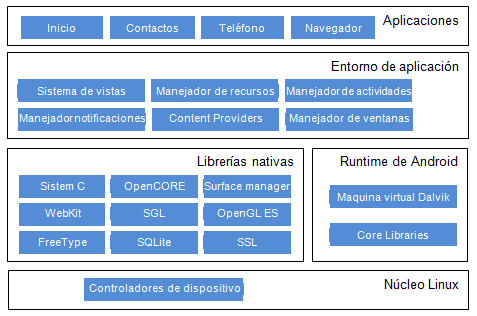
\includegraphics[width=0.75\textwidth]{figuras/docx/arquitectura-android.png}
    \caption{Arquitectura de Android (Gómez A. A., 2015)}
    \label{fig:arquitectura-android}
\end{figure}

\subsection{Ventajas y limitaciones}

Android destaca por que ofrece ventajas como:

\begin{itemize}
    \item Flexibilidad para funcionar en múltiples tipos de hardware.
    \item Libertad de personalización de interfaz.
    \item Libertad de configuración del sistema.
    \item Compatibilidad amplia con una gran variedad de herramientas y
    servicios de Google.
    \item Alta calidad de gráficos y sonido.
    \item Portabilidad garantizada, ya que sus aplicaciones son desarrolladas en
    Java.
    \item Nivel de seguridad aceptable.
\end{itemize}

Sin embargo, esto también genera limitaciones, como la fragmentación entre
dispositivos y diferentes velocidades en la distribución de actualizaciones del
sistema.

% =====================================================================
\section{Realidad Aumentada}
\label{sec:realidad-aumentada}

La realidad aumentada (RA) es una combinación visual de elementos reales y
virtuales que interaccionan entre ellos (Navarro, Martínez, \& Martínez, 2018),
también es la integración en tiempo real de la información digital en el
entorno de un usuario. La tecnología de RA superpone el contenido al mundo
real, lo que enriquece la percepción de la realidad del usuario en lugar de
reemplazarla (Hayes \& Downie, 2025). A diferencia de la realidad virtual, que
sustituye completamente el entorno físico, la RA superpone información digital
como imágenes, modelos 3D, texto o animaciones sobre la realidad observada a
través de dispositivos como smartphones, tablets o lentes inteligentes (Azuma,
1997).

\subsection{Componentes de un sistema de Realidad Aumentada}

Un sistema de Realidad Aumentada es una convergencia de hardware y software que
opera un bucle continuo de retroalimentación, en otras palabras, un sistema de
RA debe cumplir con tres características principales, combinar lo real y lo
virtual, operar interactivamente y registrar elementos en 3D (Azuma, 1997).

Un sistema de RA incluye los siguientes componentes esenciales:

\begin{itemize}
    \item \textbf{Dispositivo de visualización:} Permite mostrar la mezcla entre
    la imagen real y los elementos virtuales. Puede ser un teléfono móvil,
    tablet, gafas inteligentes o pantalla montada en la cabeza (Head-Mounted
    Display).
    \item \textbf{Cámara o sensores de captura:} Registra el entorno físico para
    detectar superficies, marcadores o puntos de referencia. Por ejemplo:
    cámaras RGB, sensores de profundidad, giroscopio, acelerómetro.
    \item \textbf{Módulo de seguimiento (tracking):} Se encarga de identificar la
    posición y orientación del usuario o del dispositivo. Esto incluye:
    marker-based, markerless, SLAM, reconocimiento de superficies.
    \item \textbf{Motor de renderizado:} Genera y superpone objetos virtuales en
    el entorno real con coherencia visual y espacial.
    \item \textbf{Interfaz de interacción:} Permite al usuario manipular objetos
    virtuales mediante gestos, toques o movimiento.
\end{itemize}

\subsection{Tecnologías para el desarrollo de Realidad aumentada móvil}

Para el desarrollo móvil, las principales tecnologías de RA son:

\begin{itemize}
    \item \textbf{ARCore:} Es el SDK de realidad aumentada de Google que ofrece
    APIs multiplataforma para crear nuevas experiencias envolventes en Android,
    iOS, Unity y la Web. Transforma la manera en que las personas juegan,
    compran, aprenden, crean y experimentan el mundo juntas mediante la
    comprensión contextual de las personas, los lugares y las cosas
    (Developers, 2025).
    \item \textbf{ARKit:} Es un framework de Apple, altamente optimizado y
    compatible con sensores avanzados como LiDAR. Permite capturar
    impresionantes videos de alta resolución perfectos para la edición de video
    profesional, producción cinematográfica, aplicaciones de redes sociales
    entre otros (Inc., 2025).
\end{itemize}

% =====================================================================
\section{Inteligencia Artificial}
\label{sec:inteligencia-artificial}

La inteligencia artificial (IA) es una tecnología transformadora que permite a
las máquinas llevar a cabo tareas de resolución de problemas similares a las de
los humanos. Desde el reconocimiento de imágenes y la generación de contenido
creativo hasta la creación de predicciones basadas en datos, la IA permite a
las empresas tomar decisiones más inteligentes a escala (Services, 2025).

La IA consiste en enseñar a las computadoras a hacer las actividades increíbles
que nuestros cerebros pueden hacer, desde comprender el mundo que las rodea
hasta aprender temas nuevos y generar ideas originales (Cloud, 2025). En el
contexto de las aplicaciones móviles, la IA permite integrar funciones
avanzadas como la personalización del contenido, la detección automática de
movimiento, el análisis de rendimiento del usuario y la interacción mediante
voz a texto.

\subsection{Aprendizaje automático}

El aprendizaje automático o Machine Learning es una subárea de la inteligencia
artificial dedicado a comprender y construir métodos para imitar la forma en
que aprenden los humanos (Pykes, 2024). El aprendizaje automático, es la
capacidad que tiene un programa para mejorar su desempeño en una tarea a partir
de la experiencia acumulada (Mitchell, 1997).

\subsection{Redes neuronales}

Una red neuronal es un programa o modelo de machine learning que toma
decisiones de forma similar al cerebro humano, al emplear procesos que imitan
la forma en que las neuronas biológicas trabajan juntas para identificar
fenómenos, sopesar opciones y llegar a conclusiones. Se basan en datos de
entrenamiento para aprender y mejorar su precisión con el tiempo (IBM, 2025).

\subsection{Visión por computadora}

La visión artificial es un campo de la inteligencia artificial, que permite a
los ordenadores y sistemas interpretar y analizar datos visuales, así como
también obtener información pertinente a partir de imágenes digitales, videos
y otros datos visuales (Cloud, 2025). En el contexto de las aplicaciones
móviles modernas, permite interpretar información visual mediante algoritmos
que detectan objetos, poses, personas entre otras características del entorno.

\subsection{Modelos de lenguaje Extenso (LLM)}

Los modelos de lenguaje, son modelos básicos entrenados sobre inmensas
cantidades de datos, lo que los hace capaces de comprender y generar lenguaje
natural y otros tipos de contenido para realizar una amplia variedad de
tareas. Por lo general, los LLM se basan en arquitecturas de aprendizaje
profundo, como Transformer, desarrollado por Google en 2017, y se pueden
entrenar con miles de millones de textos y otros tipos de contenido.

Debido a su escalabilidad, los LLM se pueden entrenar con otros tipos de datos,
como código, imágenes, audio y video, entre otros (Cloud, 2025). Su
versatilidad y capacidad de aprendizaje los convierten en herramientas clave en
el desarrollo de aplicaciones modernas, incluyendo sistemas móviles
inteligentes y soluciones que integren realidad aumentada e inteligencia
artificial.

% =====================================================================
\section{Fundamentos del entrenamiento físico}
\label{sec:entrenamiento}

\subsection{Entrenamiento físico}

El entrenamiento es un conjunto de ejercicios y actividades que se realizan
regularmente para mejorar la salud y el estado físico de una persona. Este tipo
de entrenamiento puede incluir variedad de actividades, cada una enfocada en
diferentes aspectos del cuerpo y objetivos personales (Orientanet, s.f.).

Hoy en día, la tecnología como sensores, aplicaciones móviles, realidad
aumentada e inteligencia artificial permiten un monitoreo exhaustivo de la
técnica y el análisis del movimiento, ofreciendo retroalimentación
personalizada en tiempo real. Estas innovaciones no solo optimizan el
rendimiento de los usuarios, sino que también garantizan que quienes están
comenzando su camino en el ejercicio puedan realizar las actividades de manera
segura y eficaz, contribuyendo de esta manera a la reducción de riesgo de
lesiones y fomentando un estilo de vida saludable.

\subsection{Principios del entrenamiento físico}

El entrenamiento físico está fundamentado en tres principios esenciales, estos
son:

\begin{itemize}
    \item \textbf{Fuerza:} Se centra en incrementar la capacidad del músculo para
    generar tensión, mediante ejercicios con resistencias progresivas. Esto no
    solo mejora el rendimiento deportivo, sino que también contribuye a la salud
    articular y la densidad ósea.
    \item \textbf{Técnica:} Implica la ejecución correcta de cada movimiento para
    maximizar los beneficios y minimizar riesgos. Una técnica adecuada asegura
    que el estímulo recae sobre los músculos deseados y evita compensaciones
    que puedan generar lesiones.
    \item \textbf{Hipertrofia:} Busca aumentar el tamaño del músculo mediante
    cargas, repeticiones y volúmenes adecuados. La hipertrofia requiere un
    equilibrio entre sobrecarga progresiva, nutrición y recuperación para
    generar crecimiento muscular efectivo.
\end{itemize}

\subsection{Biomecánica básica}

La biomecánica estudia el movimiento del cuerpo humano aplicando principios
mecánicos. Comprenderla permite optimizar los ejercicios, analizar palancas,
ángulos de articulaciones y fuerza aplicada, lo que mejora la eficiencia y
reduce el riesgo de lesiones. Los aspectos clave incluyen la alineación
corporal, el centro de gravedad, estabilidad y amplitud de movimiento.

La biomecánica proporciona las bases para corregir patrones de movimiento
disfuncionales, los cuales pueden surgir por hábitos sedentarios,
desequilibrios musculares o mala ejecución repetida de ejercicios. Identificar
estos patrones permite intervenir de manera temprana mediante correcciones
técnicas, fortalecimiento de músculos estabilizadores o ajustes en la postura.

\subsection{Lesiones comunes por mala técnica}

La técnica incorrecta en la ejecución de ejercicios, es una de las principales
causas de las lesiones en entornos de entrenamiento físico, especialmente en
principiantes. La evidencia científica demuestra que una postura inadecuada, la
falta de control motor y el uso de cargas excesivas incrementan el riesgo de
daño musculoarticular (Kolt \& Snyder-Mackler, 2007).

El desconocimiento de la técnica o la negligencia en la postura pueden provocar
lesiones frecuentes, como:

\begin{itemize}
    \item Dolor lumbar por levantamiento incorrecto de peso.
    \item Tendinitis por movimientos repetitivos sin control.
    \item Esguinces o distensiones musculares por falta de calentamiento o
    postura incorrecta.
    \item Lesiones articulares en hombros, rodillas o muñecas por sobrecarga o
    ángulos inadecuados.
\end{itemize}

Prevenir estas lesiones requiere educación, supervisión y el uso de tecnologías
de monitoreo como sensores de movimiento y análisis de video.

\subsection{Máquinas de gimnasio}

Una máquina de gimnasio es un equipo diseñado para facilitar la realización de
ejercicios físicos de manera controlada, segura y específica. Estas máquinas
están construidas con estructuras metálicas, poleas, cables, placas de peso o
mecanismos electrónicos que permiten guiar el movimiento del usuario. Su diseño
busca aislar determinados grupos musculares, mejorar la estabilidad durante el
ejercicio y proporcionar una carga regulable para adaptarse al nivel de cada
persona.

Las máquinas de gimnasio sirven para entrenar diferentes capacidades físicas
como fuerza, resistencia muscular, estabilidad y acondicionamiento
cardiovascular. Proporcionan un entorno controlado donde el usuario puede
ejecutar movimientos guiados que reducen el riesgo de lesiones, especialmente
en personas principiantes o en rehabilitación. También permiten trabajar grupos
musculares específicos con mayor precisión, mejorar la postura durante el
ejercicio y mantener una progresión segura mediante cargas ajustables. Además,
algunas máquinas monitorean parámetros como ritmo cardíaco, velocidad o
calorías, facilitando el seguimiento del rendimiento.

Las máquinas de gimnasio pueden clasificarse de diversas formas, pero las
categorías más comunes son:

\begin{itemize}
    \item \textbf{Según su función principal}
    \begin{itemize}
        \item \textit{Máquinas de fuerza o resistencia:} utilizan poleas,
        cables, placas de peso o sistemas hidráulicos para trabajar grupos
        musculares específicos. Ejemplos: prensa de piernas, máquina de pecho,
        jalón al pecho, curl de bíceps.
        \item \textit{Máquinas cardiovasculares:} diseñadas para mejorar la
        resistencia cardiorrespiratoria y quemar calorías. Ejemplos:
        caminadoras, bicicletas estáticas, elípticas, remadoras.
    \end{itemize}
    \item \textbf{Según el tipo de movimiento}
    \begin{itemize}
        \item \textit{Movimiento guiado:} la máquina controla la trayectoria
        del movimiento. Son ideales para principiantes.
        \item \textit{Movimiento libre asistido:} permiten mayor libertad, pero
        brindan estabilidad adicional.
    \end{itemize}
    \item \textbf{Según el mecanismo de resistencia}
    \begin{itemize}
        \item Placas de peso (weight stack): se selecciona la carga con un
        pasador.
        \item Peso libre integrado: discos que se colocan manualmente.
        \item Sistema hidráulico: resistencia generada por pistones de aire o
        aceite.
        \item Electromagnéticas: comunes en máquinas cardiovasculares modernas.
    \end{itemize}
    \item \textbf{Según el área del cuerpo que trabajan}
    \begin{itemize}
        \item Máquinas para tren superior: pecho, espalda, hombros, brazos.
        \item Máquinas para tren inferior: piernas, glúteos.
        \item Máquinas para core: abdominales, zona lumbar.
    \end{itemize}
\end{itemize}

% =====================================================================
\section{Plataforma de desarrollo}
\label{sec:plataforma}

\subsection{Visual Studio Code}

\begin{center}
    
\includegraphics[width=2.2cm]{figuras/docx/vscode-logo.png}
\end{center}

Visual Studio Code es un editor de código fuente creado por Microsoft,
diseñado para ser ligero, rápido y altamente personalizable (Cuadrado, 2022).
Sirve para escribir, corregir y organizar programas en muchos lenguajes como
Java, Python, C++, entre otros. Este funciona en Windows, Mac y Linux.

A diferencia de un IDE tradicional que viene completo desde la instalación, VS
Code parte de un núcleo ligero y va incorporando funcionalidad mediante
extensiones, lo que permite adaptarlo a prácticamente cualquier lenguaje o
framework sin cargar con herramientas que el proyecto no necesita.

\begin{figure}[H]
    \centering
    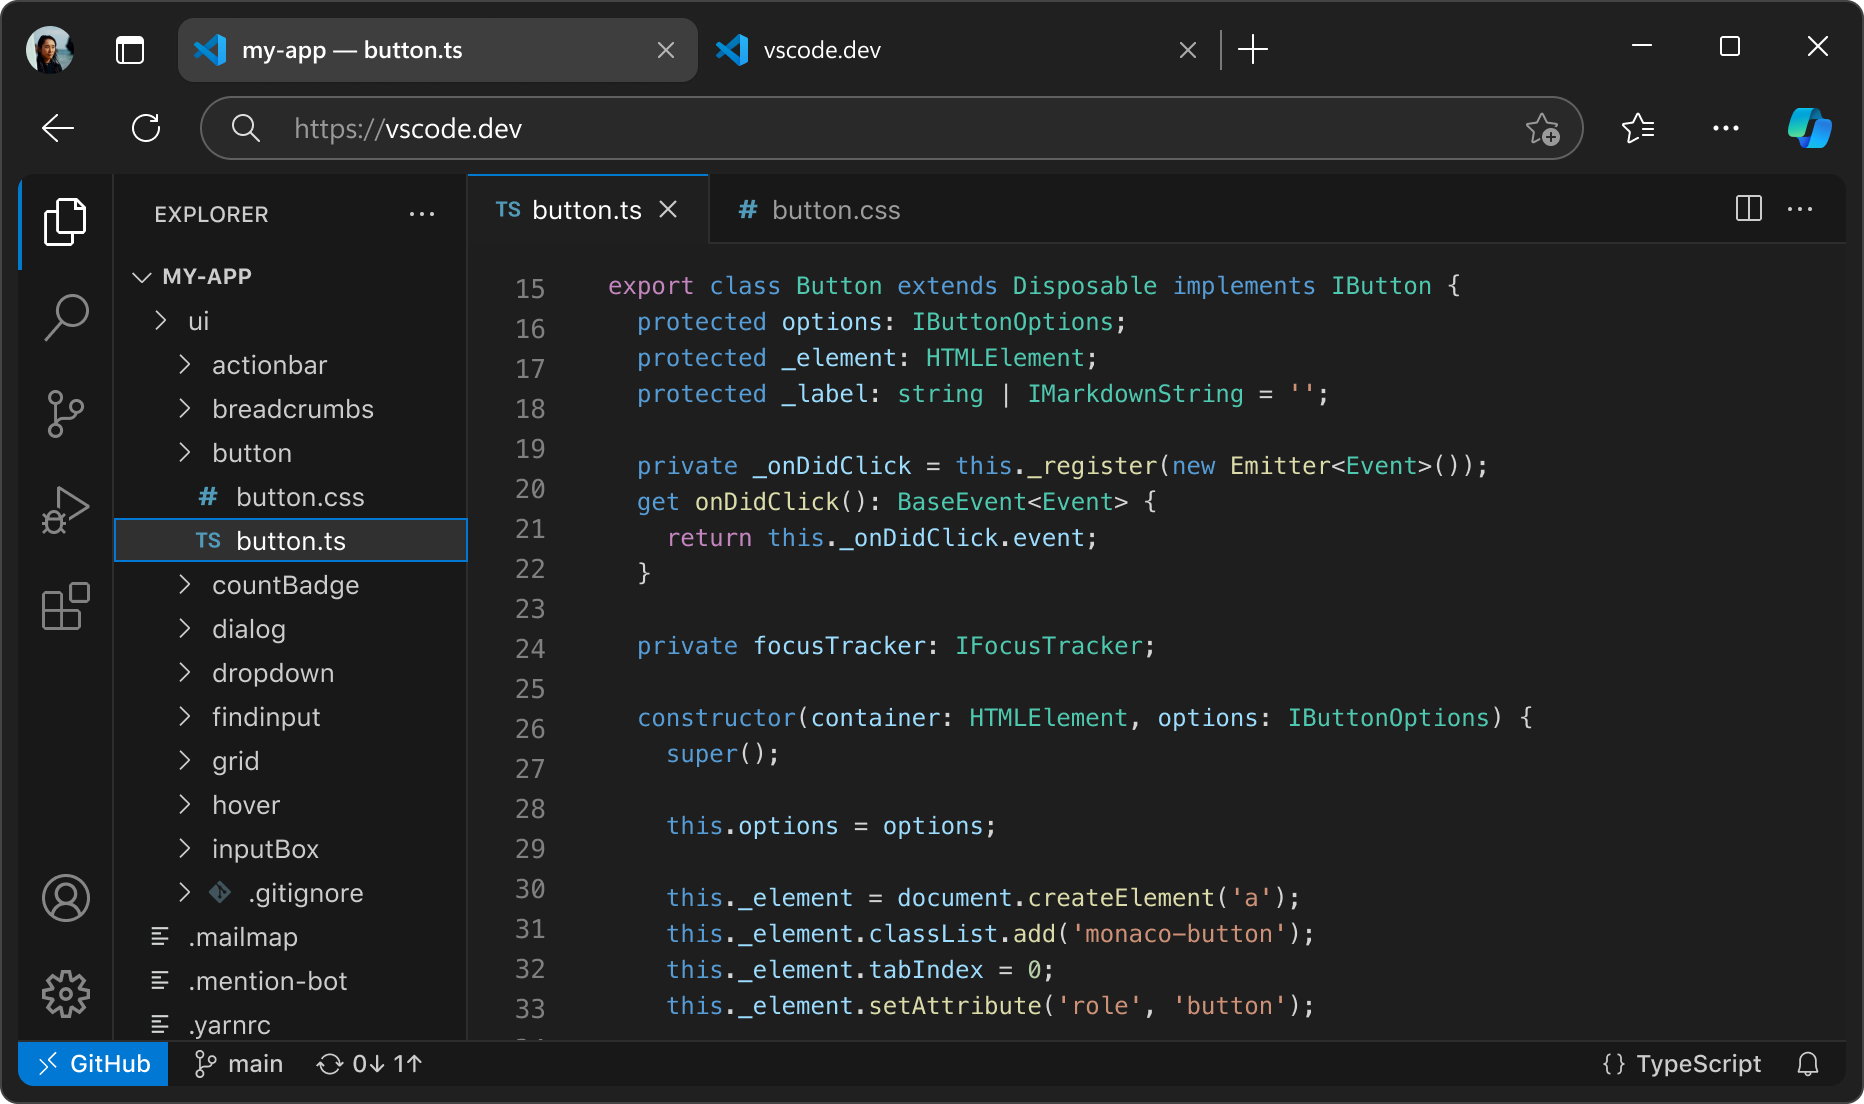
\includegraphics[width=0.85\textwidth]{figuras/docx/vscode-interfaz.png}
    \caption{Interfaz de Visual Studio Code}
    \label{fig:vscode}
\end{figure}

% =====================================================================
\section{Frameworks para desarrollo Mobile}
\label{sec:frameworks}

El desarrollo de aplicaciones móviles ha evolucionado en gran manera gracias a
la aparición de frameworks que permiten crear interfaces eficientes,
multiplataforma y optimizadas para dispositivos con recursos limitados. Estos
frameworks ofrecen herramientas, bibliotecas y entornos de trabajo que
simplifican el proceso de creación de aplicaciones al abstraer componentes
nativos y proporcionar estructuras reutilizables.

Entre los frameworks más utilizados se encuentran React Native, Flutter, Ionic,
Xamarin y Jetpack Compose.

{\small
\begin{longtable}{L{2.2cm} L{5.7cm} L{3.8cm} L{2.7cm}}
\caption{Comparación de frameworks de desarrollo Mobile}
\label{tab:frameworks}\\
\toprule
\textbf{Framework} & \textbf{Descripción} & \textbf{Características} &
\textbf{Ventajas} \\
\midrule
\endfirsthead
\toprule
\textbf{Framework} & \textbf{Descripción} & \textbf{Características} &
\textbf{Ventajas} \\
\midrule
\endhead
\bottomrule
\endfoot
React Native & Es un framework de Meta para construir aplicaciones nativas
para iOS y Android, usando JavaScript. Este framework usa el paradigma
fundamental de construcción de bloques de UI (componentes visuales con los que
interacciona el usuario) (Deloitte, 2019). &
\begin{tablista}
  \item Multiplataforma.
  \item Fast Refresh y Hot Reload.
  \item Acceso a componentes y APIs nativas.
  \item Gran comunidad y ecosistema amplio.
  \item Integración con librerías como Redux, Axios, Firebase.
\end{tablista} &
Alto rendimiento. Reutilización de código. Amplia compatibilidad. \\
\midrule
Flutter & Es un framework de código abierto de Google basado en Dart con motor
de render propio (Flutter, s.f.). &
\begin{tablista}
  \item Widgets personalizables.
  \item Animaciones.
  \item Hot Reload.
\end{tablista} &
UI consistente. Excelente rendimiento gráfico. \\
\midrule
Ionic & Ionic es un framework híbrido basado en tecnologías web (HTML, CSS,
JavaScript) que funciona mediante WebView. Permite construir aplicaciones con
enfoques multiplataforma usando Angular, React o Vue. Es especialmente útil
para aplicaciones orientadas a contenidos web o prototipado rápido (Ionic
Documentation, 2023). &
\begin{tablista}
  \item Multi-framework.
  \item Amplia colección de componentes UI.
  \item Soporte para Progressive Web Apps.
\end{tablista} &
Desarrollo rápido. Curva de aprendizaje baja. \\
\midrule
Xamarin & Xamarin es un framework de Microsoft basado en C\# y .NET, que
compila aplicaciones nativas para Android, iOS y Windows. Permite compartir
hasta 90\,\% de la lógica de negocio entre plataformas y se integra
profundamente con Visual Studio. Es utilizado ampliamente en entornos
empresariales (Microsoft, 2022). &
\begin{tablista}
  \item Acceso directo a APIs nativas.
  \item Integración con Visual Studio.
  \item Integración con .NET MAUI.
\end{tablista} &
Sólido para apps empresariales. Reutilización de lógica. \\
\midrule
Jetpack Compose & Jetpack Compose es el framework declarativo moderno de
Android, basado en Kotlin. Permite construir interfaces de usuario mediante
funciones composables, eliminando XML y ofreciendo mayor control del sistema y
rendimiento nativo. Es el estándar actual para desarrollar aplicaciones Android
modernas (Android Developers, 2024). &
\begin{tablista}
  \item UI declarativa.
  \item Integración con Android Jetpack.
  \item Animaciones avanzadas.
\end{tablista} &
Rendimiento máximo. Control total del sistema. \\
\end{longtable}
}
\fuente{Elaboración propia basada en (Deloitte, 2019); (Flutter, s.f.);
(Android Developers, 2024); (Microsoft, 2022).}

\conclusion{En conclusión, React Native destaca frente a los demás frameworks
debido a su equilibrio entre rendimiento y desarrollo multiplataforma, su
capacidad de generar componentes nativos le da mayor fluidez a diferencia de
Ionic y Flutter. Así también, permite desarrollar aplicaciones de forma
eficiente y se adapta al entorno de Android.}

\subsection{React Native}

React Native es un framework para la creación de aplicaciones nativas para iOS
y Android, creado por Meta (Facebook). Permite construir aplicaciones
multiplataforma utilizando JavaScript y React. A diferencia de las soluciones
híbridas tradicionales, React Native genera interfaces nativas, lo que permite
lograr un rendimiento cercano al desarrollo completamente nativo (React Native,
2025).

React Native se caracteriza por (Viera, s.f.):

\begin{itemize}
    \item \textbf{Componentes nativos:} Usa componentes de interfaz de usuario
    nativo en lugar de componentes web.
    \item \textbf{Hot reloading:} Permite ver cambios en tiempo real sin
    recompilar toda la app, acelerando el desarrollo.
    \item \textbf{Acceso a APIs nativas:} Permite integrar funcionalidades como
    cámara, GPS y notificaciones directamente del dispositivo.
    \item \textbf{Desarrollo Multiplataforma:} Escribe una sola vez y ejecuta en
    ambas plataformas (iOS y Android).
    \item \textbf{Gran Comunidad:} Amplia comunidad de desarrolladores y recursos
    disponibles.
    \item \textbf{Rendimiento:} Ofrece un rendimiento cercano al nativo gracias a
    su arquitectura.
    \item \textbf{Interfaz de Usuario:} Permite crear interfaces de usuario ricas
    y fluidas.
    \item \textbf{Integración con Librerías:} Compatible con librerías de
    terceros y APIs nativas.
    \item \textbf{Soporte para TypeScript:} Permite usar TypeScript para un
    desarrollo más robusto y seguro.
\end{itemize}

% =====================================================================
\section{Bases de datos de aplicaciones Móviles}
\label{sec:bases-datos}

Las bases de datos desempeñan un papel fundamental en el desarrollo de
aplicaciones móviles, ya que permiten almacenar, administrar y sincronizar la
información que utiliza el sistema durante su funcionamiento.

En el entorno móvil actual existen múltiples opciones tecnológicas, entre las
cuales destacan Firebase Firestore, SQLite, MongoDB Atlas, MySQL y PostgreSQL.

{\small
\begin{longtable}{L{2.1cm} L{5.6cm} L{3.5cm} L{3.2cm}}
\caption{Comparación de bases de datos para aplicaciones móviles}
\label{tab:bases-datos}\\
\toprule
\textbf{Base de Datos} & \textbf{Descripción} & \textbf{Características} &
\textbf{Ventajas} \\
\midrule
\endfirsthead
\toprule
\textbf{Base de Datos} & \textbf{Descripción} & \textbf{Características} &
\textbf{Ventajas} \\
\midrule
\endhead
\bottomrule
\endfoot
Firebase Firestore & Es una base de datos NoSQL en la nube que permite
sincronización en tiempo real y almacenamiento distribuido (Isaac, 2025). Su
base de datos principal, Cloud Firestore, es una solución NoSQL escalable
diseñada para sincronización en tiempo real, rendimiento móvil y arquitectura
serverless. &
\begin{tablista}
  \item Escalable.
  \item Documentos y colecciones.
  \item Soporte offline.
\end{tablista} &
\begin{tablista}
  \item Fácil integración móvil.
  \item Sin servidor.
  \item Arquitectura serverless.
  \item Integración con el ecosistema de Google.
\end{tablista} \\
\midrule
SQLite & Es una biblioteca en lenguaje C, es el motor de base de datos más
utilizado en el mundo. Se encuentra integrado en todos los teléfonos móviles y
en la mayoría de las computadoras, es de código abierto (SQLite Consortium,
2024). &
\begin{tablista}
  \item Escalable.
  \item Documentos y colecciones.
  \item Soporte offline.
\end{tablista} &
\begin{tablista}
  \item Fácil integración móvil.
  \item Ligera y de bajo consumo.
  \item Amplio soporte y estabilidad.
  \item Sin servidor.
  \item Tiempo real.
\end{tablista} \\
\midrule
MongoDB Atlas & Es un servicio de base de datos multicloud, simplifica la
implementación y gestión de bases de datos. Permite manejar grandes volúmenes
de datos, consultas avanzadas y procesamiento en la nube con altos niveles de
seguridad y escalabilidad (MongoDB, 2024) (Huang, 2020). &
\begin{tablista}
  \item Ligero.
  \item Transaccional.
  \item Estructura relacional.
\end{tablista} &
\begin{tablista}
  \item Ideal para uso offline.
  \item Ampliamente soportado.
  \item Integración nativa con la nube.
  \item Funciones avanzadas de seguridad.
\end{tablista} \\
\midrule
MySQL & MySQL es un sistema de gestión de bases de datos relacional (RDBMS) de
código abierto ampliamente utilizado en aplicaciones web y móviles.
Originalmente desarrollado por MySQL AB y actualmente mantenido por Oracle
Corporation, MySQL se ha consolidado como una solución flexible, rápida y
confiable para gestionar datos estructurados (DuBois, 2013); (Corporation,
2024). &
\begin{tablista}
  \item Lenguaje SQL para definición y manipulación de datos.
  \item Soporte para múltiples motores de almacenamiento.
  \item Ejecución de transacciones ACID.
  \item Alta compatibilidad con lenguajes de programación.
\end{tablista} &
\begin{tablista}
  \item Flexible.
  \item Escalable.
  \item Adecuada para grandes volúmenes.
\end{tablista} \\
\midrule
PostgreSQL & Sistema de gestión de bases relacional ampliamente utilizado.
Destaca por su arquitectura orientada a objetos, su capacidad para manejar
grandes volúmenes de datos y su soporte para consultas complejas, extensiones y
tipos de datos personalizados. &
\begin{tablista}
  \item SQL.
  \item Robusto.
  \item Seguro.
  \item Gestión avanzada de concurrencia.
  \item Soporte para JSON y JSONB para datos semiestructurados.
\end{tablista} &
\begin{tablista}
  \item Ideal para Backend estructurado.
  \item Rendimiento estable.
  \item Perfecto para aplicaciones móviles.
\end{tablista} \\
\end{longtable}
}
\fuente{Elaboración basada en (Corporation, 2024); (Huang, 2020); (MongoDB,
2024).}

\conclusion{En conclusión, Firebase Firestore es la mejor alternativa, por su
arquitectura NoSQL, reduce la complejidad del Backend y es escalable.}

\subsection{Firebase}

Firebase es una plataforma en la nube desarrollada por Google, facilita el
desarrollo de aplicaciones, bases de datos en tiempo real, autenticación y
hosting. Esta herramienta permite enviar notificaciones push y analizar el
rendimiento de las apps (Isaac, 2025).

En la actualidad, Firebase integra servicios modernos como Cloud Firestore,
Google Analytics 4, App Check, Data Connect y Firebase Studio, lo que la
convierte en una solución completa para proyectos actuales que buscan
escalabilidad, seguridad y analítica avanzada (López Mora, 2025).

% =====================================================================
\section{Modelos de Lenguaje Extenso (LLM)}
\label{sec:llm}

{\small
\begin{longtable}{L{2.2cm} L{4.4cm} L{4.0cm} L{3.8cm}}
\caption{Comparación de modelos de lenguaje extenso}
\label{tab:llm}\\
\toprule
\textbf{Modelo} & \textbf{Descripción} & \textbf{Características} &
\textbf{Ventajas} \\
\midrule
\endfirsthead
\toprule
\textbf{Modelo} & \textbf{Descripción} & \textbf{Características} &
\textbf{Ventajas} \\
\midrule
\endhead
\bottomrule
\endfoot
OpenAI GPT-4 & Modelo avanzado de OpenAI con capacidades de razonamiento y
comprensión contextual profunda. & Alta precisión; multimodal; entrenado con
gran cantidad de parámetros. & Respuestas coherentes; excelente para tareas
complejas. \\
\midrule
Gemini (Google) & Modelo multimodal de Google capaz de procesar texto, imágenes
y audio. & Optimización contextual; integración nativa con Google. & Muy
rápido; fuerte rendimiento en análisis multimodal. \\
\midrule
Claude 3 & Modelo de Anthropic centrado en seguridad y precisión. &
Entrenamiento ético; respuestas estables y seguras. & Ideal para tareas largas
y análisis profundo. \\
\midrule
Llama 3 & Modelo open-source de Meta, altamente eficiente y adaptable. & Open
source; optimización local; adaptable. & Perfecto para personalización y
despliegue en servidores propios. \\
\end{longtable}
}
% TODO: en el documento Word esta tabla no tenía fila de "Fuente".
\fuente{\pendiente{indicar la fuente de la tabla.}}

\subsection{OpenAI}

OpenAI ofrece modelos de lenguaje avanzados, como GPT-4, que permiten realizar
tareas complejas de procesamiento de lenguaje natural, generación de texto,
análisis semántico, recomendaciones personalizadas y soporte conversacional.
Estos modelos se integran mediante API y pueden ser empleados dentro de
aplicaciones móviles para funciones inteligentes.

Los modelos de OpenAI están basados en la arquitectura Transformer, que permite
procesar grandes volúmenes de información con alta precisión. Además, OpenAI
proporciona herramientas que facilitan la integración de estos modelos en
distintos entornos tecnológicos, incluyendo plataformas web, sistemas de
atención al cliente, análisis de datos y automatización de procesos
empresariales. Los modelos aprenden a partir de enormes conjuntos de datos, lo
que les permite comprender contextos complejos, mantener conversaciones
coherentes y generar contenido creativo en múltiples idiomas. Por otra parte,
OpenAI trabaja en la mejora continua de la seguridad y la ética en el uso de
IA, implementando mecanismos para minimizar sesgos, evitar desinformación y
garantizar que los resultados sean confiables y útiles para los usuarios
finales.

% =====================================================================
\section{Herramientas}
\label{sec:herramientas}

\subsection{Control de versiones}

El control de versiones es un sistema que ayuda a rastrear y gestionar los
cambios realizados en un archivo o conjunto de archivos, principalmente
utilizado por ingenieros de software para hacer seguimiento a las
modificaciones realizadas en el código fuente (B, 2025).

Para esto utilizaremos:

\begin{enumerate}
    \item \textbf{Git:} Es un sistema de control de versiones distribuido,
    gratuito y de código abierto diseñado para manejar proyectos pequeños, como
    también proyectos muy grandes de forma rápida y eficiente (Git, s.f.).
    \item \textbf{GitHub:} Es un servicio basado en la nube que aloja un sistema
    de control de versiones (VCS) llamado Git. Éste permite a los
    desarrolladores colaborar y realizar cambios en proyectos compartidos, a la
    vez que mantienen un seguimiento detallado de su progreso (B, 2025).
\end{enumerate}

\subsection{Herramientas de Gestión}

Las herramientas de gestión de proyectos están especialmente diseñadas para
asistir a un empleado o equipo en la gestión eficaz de sus proyectos y tareas
(Gurnov \& Wrike (W.), 2025). Estas herramientas son utilizadas para la
organización, planificación, seguimiento y aseguramiento de calidad del
proyecto.

\begin{itemize}
    \item \textbf{Trello:} Es una herramienta flexible para la gestión del
    trabajo, basado en tableros Kanban que facilita la organización visual de
    tareas mediante listas y tarjetas (Atlassian, 2023). Su enfoque intuitivo
    permite coordinar actividades, asignar responsabilidades y monitorear el
    avance de cada fase del proyecto.
\end{itemize}

\chapter{ÁREA DE APLICACIÓN}
\label{cap:area-aplicacion}

El presente capítulo describe el enfoque metodológico adoptado para el
desarrollo del sistema inteligente de entrenamiento en gimnasios con realidad
aumentada e inteligencia artificial. El propósito es garantizar un proceso de
construcción ordenado, iterativo y orientado a la calidad, acorde a las
necesidades específicas del desarrollo móvil. Para ello, se selecciona la
metodología ágil Mobile-D, diseñada especialmente para proyectos móviles con
ciclos de producción rápidos, entregas frecuentes y constante
retroalimentación.

% =====================================================================
\section{Antecedentes}
\label{sec:aa-antecedentes}

\subsection{Enfoque metodológico}

La metodología es el conjunto de procedimientos, técnicas y estrategias que
orienta la ejecución de un proyecto de investigación o desarrollo tecnológico.
En el presente trabajo, el enfoque metodológico define la manera en que se
estructura el proceso de diseñar, desarrollar y evaluar el sistema. El proyecto
adopta un enfoque cuantitativo-aplicado porque se medirá métricas objetivas del
sistema inteligente, como también se realizará la creación de una solución
tecnológica concreta mediante el uso de técnicas de ingeniería de software,
inteligencia artificial y realidad aumentada. En este caso, se emplean
fundamentos de biomecánica, visión por computadora, aprendizaje automático y
diseño de software para desarrollar una herramienta que facilite el uso
correcto de máquinas, la corrección técnica de ejercicios y la personalización
del entrenamiento.

% =====================================================================
\section{Metodología de desarrollo}
\label{sec:aa-metodologia}

La metodología Mobile-D fue seleccionada para guiar el proceso de desarrollo
del sistema debido a que está específicamente diseñada para proyectos de
software orientados a dispositivos móviles, caracterizados por ciclos de
producción rápidos, restricciones de hardware y cambios frecuentes en los
requerimientos.

Mobile-D es una metodología ágil diseñada para el desarrollo de aplicaciones
móviles, que requiere ciclos de entrega cortos, validación continua, pruebas en
dispositivos reales y flexibilidad ante cambios de interfaz o funcionalidad. El
presente proyecto integra módulos de guía interactiva mediante imágenes,
animaciones o realidad aumentada, generación de rutinas personalizadas mediante
inteligencia artificial, herramientas de seguimiento físico y una interfaz
altamente intuitiva.

Mobile-D permite abordar de forma progresiva y controlada, los elementos
principales del proyecto:

\begin{itemize}
    \item La guía visual sobre el uso correcto de máquinas y la ejecución de
    ejercicios, que exige pruebas de usabilidad desde las primeras etapas.
    \item La generación de rutinas personalizadas mediante algoritmos de IA,
    cuya precisión y utilidad deben ajustarse iterativamente.
    \item Los módulos de planificación y seguimiento, que requieren
    refinamientos sucesivos para asegurar claridad, funcionalidad y coherencia
    en la experiencia del usuario.
    \item La interfaz móvil, que debe ser evaluada continuamente para
    garantizar facilidad de uso, accesibilidad y entendimiento para usuarios
    principiantes.
\end{itemize}

% =====================================================================
\section{Aplicación de la Metodología Mobile-D}
\label{sec:aa-aplicacion-mobiled}

La metodología Mobile-D se implementa en el presente proyecto mediante cinco
fases que permiten estructurar el desarrollo de la aplicación de manera
incremental, verificable y orientada a la calidad. A continuación, se detalla
la aplicación específica de cada fase al sistema inteligente de entrenamiento.

% ---------------------------------------------------------------------
\subsection{Fase de Exploración}

En esta etapa se definen las bases conceptuales, técnicas y organizativas del
presente proyecto.

\titulillo{Módulos principales del sistema}

El sistema propuesto está compuesto por los siguientes módulos esenciales:

\begin{itemize}
    \item Registro y autenticación de usuarios.
    \item Guía detallada del uso correcto de máquinas de gimnasio.
    \item Ejecución técnica correcta de ejercicios específicos.
    \item Rutinas personalizadas mediante inteligencia artificial.
    \item Registro nutricional básico (calorías diarias).
    \item Seguimiento del progreso físico (peso, IMC, medidas).
    \item Reportes estadísticos y visualización del avance.
\end{itemize}

\titulillo{Requerimientos de sistema}

\textit{Requerimientos Funcionales}

\begin{itemize}
    \item RF1: Registrar y autenticar usuarios mediante correo y contraseña.
    \item RF2: Mostrar información técnica y visual de cada máquina de gimnasio.
    \item RF3: Generar rutinas personalizadas mediante IA según edad, peso, nivel
    y objetivo.
    \item RF4: Registrar peso, estatura, IMC y progreso físico.
    \item RF5: Registrar ingesta calórica diaria del usuario.
    \item RF6: Visualizar reportes y estadísticas del progreso físico.
\end{itemize}

\textit{Requerimientos No Funcionales}

\begin{itemize}
    \item RNF1: La aplicación debe ejecutarse en Android versión 8.0 o superior.
    \item RNF2: La interfaz debe ser intuitiva, rápida y adaptable a diferentes
    pantallas.
    \item RNF3: La sincronización de datos debe realizarse en tiempo real
    mediante Firebase.
\end{itemize}

\titulillo{Selección de Tecnologías}

\textit{Frontend}

\begin{itemize}
    \item \textbf{React Native:} Es un framework multiplataforma, que permite
    desarrollar aplicaciones móviles para dispositivos Android.
    \item \textbf{JavaScript:} Lenguaje de programación principal para el
    desarrollo de las interfaces y la lógica del lado del cliente.
    \item \textbf{Figma:} Herramienta de diseño utilizada para crear prototipos
    interactivos, pantallas iniciales, facilitando la validación visual del
    producto.
\end{itemize}

\textit{Backend}

\begin{itemize}
    \item \textbf{Firebase Authentication:} Servicio que permite gestionar el
    registro, inicio de sesión y recuperación de credenciales de forma segura.
    \item \textbf{Firebase Firestore:} Base de datos NoSQL en la nube que
    proporciona sincronización en tiempo real y escalabilidad para manejar
    información de usuarios, ejercicios, rutinas y progreso.
    \item \textbf{Firebase Storage:} Servicio destinado al almacenamiento de
    imágenes, animaciones y videos que acompañan la guía técnica del sistema.
    \item \textbf{TensorFlow Lite:} Biblioteca optimizada para ejecutar modelos
    de inteligencia artificial directamente en el dispositivo móvil, utilizada
    para generar rutinas personalizadas basadas en parámetros del usuario.
\end{itemize}

% ---------------------------------------------------------------------
\subsection{Fase de Inicialización}

En esta fase se prepara el entorno de desarrollo, la planificación inicial y la
definición de la arquitectura del sistema. También se establecen los
lineamientos de codificación y los mecanismos de control de versiones (Git).

\titulillo{Configuración del entorno}

Las principales actividades a realizar para la preparación del ambiente, son:

\begin{itemize}
    \item Instalación de Node.js.
    \item Instalación de Expo CLI.
    \item Creación de proyecto en Firebase y configuración de los servicios de
    autenticación, Firestore y Storage.
    \item Integración de la librería de TensorFlow Lite.
    \item Creación del repositorio en GitHub y definición de las ramas
    principales.
\end{itemize}

\titulillo{Arquitectura del sistema}

La arquitectura definida para el desarrollo de la aplicación es el de
cliente-servidor, donde la aplicación móvil actúa como cliente y los servicios
en la nube proporcionan autenticación, almacenamiento de datos, persistencia
multimedia y ejecución de algoritmos de IA.

La arquitectura cliente servidor permite garantizar escalabilidad,
sincronización en tiempo real y disponibilidad permanente del servicio.

\titulillo{Estructura de la arquitectura}

La estructura de la arquitectura del sistema se encuentra basada en capas:

\paragraph{Capa de Presentación}

Tecnologías: React Native + Expo, JavaScript, componentes UI.

\textit{Responsabilidades:}

\begin{itemize}
    \item Generar la interfaz visual de la aplicación.
    \item Gestionar la interacción del usuario.
    \item Capturar entradas como datos personales, selección de máquinas,
    rutinas y registro nutricional.
    \item Comunicar solicitudes al backend y mostrar respuestas.
\end{itemize}

\textit{Componentes clave:}

\begin{itemize}
    \item Módulo de registro y autenticación.
    \item Módulo de guía de máquinas y ejercicios.
    \item Módulo de rutinas personalizadas.
    \item Módulo de nutrición.
    \item Módulo de progreso y reportes.
\end{itemize}

\paragraph{Capa de Lógica de Negocio}

Esta se encuentra dentro de la app y está conectada a servicios externos.

\textit{Responsabilidades:}

\begin{itemize}
    \item Manejar reglas del sistema (cálculo de IMC, validaciones).
    \item Procesar datos antes de enviarlos a Firebase.
    \item Integrar y ejecutar modelos TensorFlow Lite para personalizar
    rutinas.
    \item Gestionar filtros, búsqueda de máquinas y procesamiento de
    ejercicios.
\end{itemize}

\textit{Componentes de negocio:}

\begin{itemize}
    \item Controlador de rutinas (IA).
    \item Controlador de ejercicios y máquinas.
    \item Controlador de progreso físico.
    \item Controlador nutricional.
\end{itemize}

\paragraph{Capa de Servicios}

Esta capa proporciona servicios esenciales para la operación del sistema:

\textit{Firebase Authentication:}

\begin{itemize}
    \item Registro de usuarios.
    \item Inicio de sesión.
    \item Recuperación de contraseñas.
    \item Seguridad y manejo de tokens.
\end{itemize}

\textit{Firebase Firestore:}

\begin{itemize}
    \item Base de datos NoSQL en tiempo real.
    \item Almacenamiento de rutinas, registros, progreso y máquinas.
\end{itemize}

\textit{Firebase Storage:}

\begin{itemize}
    \item Almacenamiento de imágenes, videos o animaciones educativas.
    \item Contenido para la guía técnica de máquinas.
\end{itemize}

\textit{Firebase Cloud Functions (opcional):}

\begin{itemize}
    \item Validación de datos.
    \item Preprocesamiento de peticiones.
    \item Actualizaciones automáticas de rutinas.
\end{itemize}

Estas funciones se integran a través de peticiones HTTP o SDK en tiempo real.

\paragraph{Capa de Inteligencia Artificial}

Tecnología: TensorFlow Lite.

\textit{Responsabilidades:}

\begin{itemize}
    \item Ejecutar modelos de recomendación ligera para rutinas.
    \item Ajustar parámetros según peso, nivel, objetivo y progreso del
    usuario.
    \item Proveer resultados inmediatos sin depender del servidor.
\end{itemize}

Este esquema reduce latencia, permite personalización offline y mejora la
experiencia del usuario.

% ---------------------------------------------------------------------
\subsection{Fase de Producción}

Esta es la etapa central del desarrollo. Dentro de esta etapa se implementan
los módulos de IA, seguimiento físico y rutinas personalizadas. Esta fase de
producción se organiza en iteraciones cortas, cada una de las cuales agrega un
conjunto de funcionalidades al sistema.

\titulillo{\textit{Día de prueba}}

En este día se verifica que toda la plataforma técnica funcione correctamente
antes de empezar a desarrollar funcionalidades reales.

Se debe realizar las siguientes acciones:

\begin{itemize}
    \item \textbf{Verificación de la integración con Firebase}

    Se realizarán pruebas básicas con los servicios principales de Firebase
    para garantizar su correcto funcionamiento:
    \begin{itemize}
        \item \textbf{Authentication:} creación de usuarios de prueba,
        validación de inicio de sesión y manejo de errores.
        \item \textbf{Firestore:} creación de colecciones temporales, escritura
        y lectura de documentos, y verificación de permisos básicos.
        \item \textbf{Storage:} carga y visualización de archivos multimedia
        para garantizar el acceso correcto al módulo de almacenamiento.
    \end{itemize}
    Estas pruebas aseguran que la aplicación pueda gestionar información real
    durante la fase de producción.
\end{itemize}

\textbf{Validación del entorno móvil}

Se verifica la correcta compilación del proyecto tanto en un dispositivo físico
como en un emulador. Además, se comprueba la navegación entre pantallas
iniciales y la ejecución estable del entorno Expo.

\textbf{Prueba preliminar del modelo TensorFlow Lite}

Se verifica la carga del modelo de inteligencia artificial y su ejecución
básica en el dispositivo, con el fin de confirmar la compatibilidad entre
TensorFlow Lite y la plataforma móvil utilizada.

\textbf{Validación del control de versiones}

Se realiza una prueba de uso del repositorio GitHub, asegurando que se pueden
subir y descargar cambios correctamente, lo cual es indispensable para mantener
un desarrollo organizado.

\titulillo{\textit{Día de salida}}

En este día se cierra la fase de inicialización, aquí no se realizan pruebas
sino ajustes finales y organización para dejar el proyecto listo para comenzar
la fase de producción.

Para esto, se debe realizar:

\textbf{Organización y limpieza del proyecto}

Se reorganiza la estructura interna del proyecto siguiendo la arquitectura
definida, agrupando componentes, servicios, pantallas y modelos de datos en
carpetas específicas. Asimismo, se eliminaron archivos temporales o de prueba
utilizados en fases previas.

\textbf{Configuración de variables y llaves de entorno}

Se definieron archivos seguros para almacenar las credenciales de Firebase y
otras configuraciones sensibles, evitando que estas sean expuestas en el
repositorio de código.

\textbf{Creación de ramas base de desarrollo en GitHub}

Se estableció una estructura de ramas para gestionar el desarrollo:

\begin{itemize}
    \item \texttt{main}: versión estable.
    \item \texttt{development}: versión en progreso.
    \item \texttt{feature/nombre-del-módulo}: para cada nueva funcionalidad.
\end{itemize}

Esta estructura permite un control ordenado de versiones.

% ---------------------------------------------------------------------
\subsection{Fase de Estabilización}

Dentro de esta fase se integran y verifican los componentes desarrollados,
asegurando consistencia, rendimiento y compatibilidad entre módulos. Las
pruebas de usabilidad y validación funcional se intensifican.

Las actividades a realizarse en esta fase son:

\begin{itemize}
    \item Refactorizar código para mejorar legibilidad.
    \item Optimizar carga de imágenes y videos.
    \item Ajustar tiempos de respuesta del sistema.
    \item Revisar el diseño visual para mejorar usabilidad.
    \item Corregir detalles detectados durante las pruebas en dispositivos
    reales.
\end{itemize}

% ---------------------------------------------------------------------
\subsection{Fase de Pruebas del sistema}

Se ejecutan pruebas de aceptación, evaluación del modelo de IA, pruebas en
dispositivos reales y corrección final de errores. El objetivo es garantizar
que el sistema sea estable y esté listo para su uso práctico.

Esto mediante las siguientes pruebas:

\begin{itemize}
    \item \textbf{Pruebas Funcionales:} Las pruebas funcionales son un tipo de
    verificación que evalúa si el sistema cumple correctamente con los
    requerimientos establecidos, las pruebas funcionales se basan en técnicas
    de caja negra, donde el evaluador verifica funciones, escenarios y
    respuestas del sistema desde la perspectiva del usuario final (IEEE, 1990).
    \item \textbf{Pruebas de Usabilidad:} Las pruebas de usabilidad se enfocan
    en analizar qué tan fácil, eficiente y satisfactoria es la interacción de un
    usuario con la interfaz del sistema. Se fundamenta en principios como
    facilidad de aprendizaje, eficiencia, reducción de errores y satisfacción
    del usuario (Nielsen, 1993).
    \item \textbf{Pruebas de Aceptación:} Las pruebas de aceptación validan que
    el sistema completo cumpla con los requerimientos acordados, estas pruebas
    representan la etapa final de validación del producto e incluyen la
    ejecución de escenarios reales que reflejan el uso cotidiano de la
    aplicación (Pressman, 2010).
\end{itemize}

% =====================================================================
\section{Roles}
\label{sec:aa-roles}

Dentro de la metodología Mobile-D, los roles cumplen la función de organizar
las responsabilidades durante el desarrollo del proyecto, aun cuando éste sea
desarrollado por una sola persona.

A continuación, se describen los roles adoptados en el proyecto:

\begin{table}[H]
\centering
\caption{Roles establecidos por Mobile-D}
\label{tab:roles}
\begin{tabularx}{\textwidth}{L{3.6cm} Y L{3cm}}
\toprule
\textbf{Rol} & \textbf{Responsabilidades} & \textbf{Responsable} \\
\midrule
Product Owner & Define alcance, objetivos y prioridades del sistema & Erika
Chino \\
Arquitecto Mobile & Diseña la arquitectura y selecciona las tecnologías & Erika
Chino \\
Desarrollador móvil & Implementa módulos, interfaces y lógica de negocio &
Erika Chino \\
Diseñador UI/UX & Diseña prototipos, navegación y experiencia de usuario &
Erika Chino \\
QA Tester & Realiza pruebas funcionales, de usabilidad y rendimiento & Erika
Chino \\
\bottomrule
\end{tabularx}
\fuente{Elaboración propia.}
\end{table}

% =====================================================================
\section{Técnicas e instrumentos de recolección de información}
\label{sec:aa-tecnicas}

Para fundamentar el diseño y funcionamiento del sistema se utilizarán las
siguientes técnicas:

\begin{itemize}
    \item \textbf{Revisión documental:} Investigación de aplicaciones similares,
    biomecánica, técnica correcta de ejercicios y libros especializados.
    \item \textbf{Observación directa:} Registro del uso real de máquinas en
    gimnasios locales.
    \item \textbf{Entrevistas informales:} Conversaciones con usuarios
    principiantes para conocer sus dificultades reales en el gimnasio.
    \item \textbf{Prototipado:} Elaboración de pantallas en Figma para validar
    la experiencia de usuario antes del desarrollo.
\end{itemize}

\chapter{DESARROLLO DEL PROYECTO}
\label{cap:desarrollo}

% En el documento Word este capítulo solo tenía el título y la primera
% sección vacía. En la carpeta borradores/capitulos/ hay una propuesta de
% redacción completa del Capítulo IV (fases de Mobile-D) basada en el código
% real de coach-app, por si se quiere usar como punto de partida.

\section{Fase de Exploración}
\label{sec:des-exploracion}

\pendiente{Desarrollar el contenido del Capítulo IV.}


% ---------------- Bibliografía ----------------
% =====================================================================
%  BIBLIOGRAFÍA (formato APA, transcrita del documento Word)
%  Cada referencia es un \item dentro del entorno referenciasapa.
% =====================================================================
\chapter*{BIBLIOGRAFÍA}
\addcontentsline{toc}{chapter}{BIBLIOGRAFÍA}
\label{cap:bibliografia}

\begin{referenciasapa}

\item Abrahamsson, P., Hanhineva, A., Hulkko, H., Ihme, T., Jäälinoja, J.,
Koskela, J., \ldots{} Salo, O. (2004). \textit{Mobile-D: An Agile Approach for
Mobile Application Development.} Helsinki: VTT Publications.

\item Alliance, O. H. (2022). Obtenido de Android Open Source Project
Overview.: \url{https://source.android.com/?hl=es-419}

\item Android Developers, G. (2024). \textit{Introducción a Android Studio}.
Obtenido de Android Developers:
\url{https://developer.android.com/studio/intro?hl=es-419}

\item Apple. (2023). \textit{Apple Developer Documentation}. Obtenido de
\url{https://developer.apple.com/}

\item AppMaster. (4 de septiembre de 2023). \textit{Programación Móvil}.
Obtenido de \url{https://appmaster.io/es/glossary/programacion-movil}

\item Apps, L. B. (2011). \textit{Guía de aplicaciones móviles.} Obtenido de
Guía de aplicaciones móviles. Fundación Telefónica.

\item Atlassian. (2023). \textit{About us: Trello history, logos \& customers
| Trello}. Obtenido de Atlassian Trello: \url{https://trello.com/about}

\item Azuma, R. (1997). \textit{A Survey of Augmented Reality.} Obtenido de
\url{https://www.cs.unc.edu/~azuma/ARpresence.pdf}

\item B, G. (13 de marzo de 2025). \textit{Qué es GitHub y cómo empezar a
usarlo}. Obtenido de ES Tutoriales:
\url{https://www.hostinger.com/es/tutoriales/que-es-github}

\item Beck, K., \& Andres, C. (2005). Extreme Programming Explained: Embrace
change. En \textit{Extreme Programming Explained.} Addison-Wesley.

\item Booch, G., Maksimchuk, R., Engel, M., Young, B., Conallen, J., \&
Houston, K. (2007). \textit{Object-Oriented Analysis and Design with
Applications.} Addison-Wesley.

\item Cloud, G. (2025). \textit{Inteligencia Artificial (IA): una guía fácil de
entender}. Obtenido de
\url{https://cloud.google.com/learn/what-is-artificial-intelligence?hl=es-419}

\item Corporation, O. (2024). \textit{MySQL Documentation}. Obtenido de MySQL:
\url{https://dev.mysql.com/doc/}

\item Cuadrado, G. C. (22 de julio de 2022). \textit{OpenWebinars}. Obtenido de
\url{https://openwebinars.net/blog/que-es-visual-studio-code-y-que-ventajas-ofrece/}

\item \textit{Curso para desarrollo de apps con React Native}. (s.f.). Obtenido
de Código Facilito: \url{https://codigofacilito.com/articulos/que-es-react-native}

\item Deloitte. (2019). \textit{¿Qué es React Native? | Tecnología | Deloitte
España}. Obtenido de Deloitte:
\url{https://www.deloitte.com/es/es/services/consulting/blogs/todo-tecnologia/que-es-react-native.html}

\item Developers, G. F. (2025). \textit{Crea nuevas experiencias de realidad
aumentada que combinen perfectamente con el mundo digital con el físico |
ARCore | Google for Developers.} Obtenido de ARCore:
\url{https://developers.google.com/ar?hl=es-419}

\item DuBois, P. (2013). \textit{MySQL.} Addison-Wesley Professional.

\item Edward Laux, J. S. (2016). Obtenido de BodBot AI Entrenador Personal:
\url{https://www.bodbot.com/}

\item Flutter, s. (s.f.). \textit{Flutter - Crea aplicaciones para cualquier
pantalla.} Obtenido de \url{https://esflutter.dev/}

\item Gabriel Maide, E., \& Pacienzia, J. (noviembre de 2020).
\textit{Metodologías de desarrollo de software aplicadas a proyectos de
automatización de procesos.} Obtenido de Pistas Educativas:
\url{https://pistaseducativas.celaya.tecnm.mx/index.php/pistas/article/viewFile/2381/1900}

\item GeeksforGeeks. (11 de julio de 2025). \textit{Incremental Process Model
Software Engineering.} Obtenido de GeeksforGeeks:
\url{https://www.geeksforgeeks.org/software-engineering/software-engineering-incremental-process-model/}

\item Gironés, T. (2012). \textit{Aplicaciones móviles: Conceptos y
desarrollo.}

\item Git. (s.f.). Obtenido de \url{http://git-scm.com/}

\item Gjestvang, C. S. (s.f.). \textit{Motives and barriers to initiation and
sustained exercise adherence in new fitness club members: A prospective study.
Publicado en Frontiers in Psychology.} Obtenido de
\url{https://psycnet.apa.org/record/2020-64605-023}

\item Global, S. (noviembre de 2025). Obtenido de Mobile Operating System Market
Share Plurinational State of Bolivia | StatCounter Global Stats:
\url{https://gs.statcounter.com/os-market-share/mobile/bolivia}

\item Gómez, \& Hernández. (2016). Mobile-D: Metodología ágil para el desarrollo
de aplicaciones móviles. \textit{Revista Orbis}.

\item Gómez, A. A. (2015). \textit{Comparación de dos tecnologías de desarrollo
de aplicaciones móviles desde la perspectiva de los atributos de calidad}.
Obtenido de ResearchGate:
\url{https://www.researchgate.net/figure/Figura-5-Arquitectura-de-Android_fig3_319975215}

\item Gómez, A. A. (2015). \textit{Comparación de dos tecnologías de desarrollo
de aplicaciones móviles desde la perspectiva de los atributos de calidad.}
Universidad Nacional de Colombia: Bogotá.

\item Google. (2023). \textit{Android Developers -- Official Documentation}.
Obtenido de \url{https://developer.android.com/}

\item Group, L. F. (2021). \textit{Ejercicios en el Gimnasio}. Obtenido de
\url{https://play.google.com/store/apps/details?id=gymworkout.gym.gymlog.gymtrainer&hl=es_BO}

\item Guide, I. S. (12 de septiembre de 2023). \textit{Modelo en espiral:
modelo de reducción de riesgos para proyectos de software.} Obtenido de
\url{https://www.ionos.mx/startupguide/productividad/modelo-en-espiral/}

\item Gurnov, A., \& Wrike (W.). (13 de noviembre de 2025). \textit{Las 21
mejores herramientas de gestión de proyectos}. Obtenido de Wrike:
\url{https://www.wrike.com/es/project-management-guide/faq/que-son-las-herramientas-de-gestion-de-proyectos/}

\item Hayes, M., \& Downie, A. (28 de noviembre de 2025). \textit{Realidad
aumentada. IBM}. Obtenido de IBM:
\url{https://www.ibm.com/es-es/think/topics/augmented-reality}

\item Huang, S. (2020). \textit{NoSQL Databases: Concepts and Applications.}
Cambridge: Morgan Kaufmann.

\item IBM. (2025). \textit{¿Qué son las redes neuronales?} Obtenido de
\url{https://www.ibm.com/es-es/think/topics/neural-networks}

\item IEEE. (1990). \textit{IEEE Standard Glossary of Software Engineering
Terminology}. Obtenido de Institute of Electrical and Electronics Engineers.

\item Inc., A. (2025). \textit{ARKit 6 - Augmented Reality - Apple Developer.}

\item Ionic Documentation, F. (2023). \textit{Ionic Framework.} Obtenido de
Ionic Documentation: \url{https://ionicframework.com/docs}

\item Isaac. (2025). \textit{Firebase: Qué es y cómo funciona la plataforma de
Google}. Obtenido de Mundobytes: \url{https://mundobytes.com/firebase-que-es/}

\item Kolt, G., \& Snyder-Mackler, L. (2007). \textit{Terapias físicas en el
deporte y el ejercicio.}

\item Leyva, R., León, G., \& García, F. (2016). Metodología Mobile-D para el
desarrollo de aplicaciones móviles. \textit{Revista Cubana de Ciencias
Informáticas, 10}(3), 45--57. Obtenido de
\url{https://www.researchgate.net/figure/Figura-210-Metodologia-Mobile-D-Fuente-Leyva-et-al-2016_fig5_348295603}

\item López Mora, S. (noviembre de 2025). \textit{Firebase: qué es, para qué
sirve, funcionalidades y ventajas}. Obtenido de DIGITAL55:
\url{https://digital55.com/blog/que-es-firebase-funcionalidades-ventajas-conclusiones/}

\item Meier, R., \& Lake, I. (2018). \textit{Professional Android} (4.ª ed.).

\item Microsoft. (2022). \textit{Xamarin Documentation}. Obtenido de Microsoft
Learn: \url{https://learn.microsoft.com/en-us/xamarin/}

\item Mitchell, T. (1997). \textit{Machine Learning.} New York: McGraw-Hill.

\item MongoDB, I. (2024). \textit{MongoDB Atlas documentation}. Obtenido de
\url{https://www.mongodb.com/docs/atlas/}

\item Navarro, F., Martínez, A., \& Martínez, J. (2018). \textit{Realidad
Virtual y Realidad Aumentada.} Ra-Ma.

\item Nielsen, J. (1993). \textit{Usability Engineering.} Academic Press.

\item Nystrom, K. (2021). \textit{Kotlin Programming: The Big Nerd Ranch Guide.
Big Nerd Ranch.} Pearson Education Store.

\item Orientanet. (s.f.). \textit{Orientanet}. Obtenido de ¿Qué es
entrenamiento físico y tipos?:
\url{https://www.orientanet.es/que-es-entrenamiento-fisico-y-tipos/}

\item Pressman, R. S. (2010). \textit{Software Engineering: A Practitioner's
Approach.} Higher Education.

\item Pykes, K. (2024). \textit{Aprendizaje automático en Python: Tutorial de
Scikit-Learn}. Obtenido de
\url{https://www.datacamp.com/es/tutorial/machine-learning-python}

\item \textit{React Native}. (2025). Obtenido de
\url{https://reactnative.dev/docs/intro-react-native-components}

\item Santander, B. (21 de diciembre de 2020). \textit{Metodologías de
desarrollo de software: ¿qué son?} Obtenido de Santander:
\url{https://www.santanderopenacademy.com/es/blog/metodologias-desarrollo-software.html}

\item Sanz, D. (2019). Obtenido de Introducción a Android:
\url{https://dspace.itsjapon.edu.ec/jspui/bitstream/123456789/434/1/introduccion-android.pdf}

\item Schwaber, K., \& Sutherland, J. (2020). \textit{The Scrum Guide: The
Definitive Guide to Scrum.} Boston: Scrum.org.

\item Services, A. W. (2025). Obtenido de ¿Qué es la IA? -- Explicación de la
inteligencia artificial -- AWS:
\url{https://aws.amazon.com/es/what-is/artificial-intelligence/}

\item Sharma, M. (2018). \textit{Productivity gains with modern IDEs: A review
of IntelliJ-based environments.}

\item Smith, J., \& Darrow, M. (2019). \textit{Gradle for Android Development.}
O'Reilly Media.

\item Sommerville, I. (2011). \textit{Software Engineering.} Boston:
Addison-Wesley.

\item SQLite Consortium. (2024). \textit{SQLite Home page}. Obtenido de
SQLite.org: \url{https://sqlite.org/}

\item Team. (2024). \textit{Metodologías de desarrollo de software: guía para
optimizar tu proyecto.} Obtenido de Blog de Desarrollo de Software, Testing e
Inteligencia Artificial | Abstracta:
\url{https://es.abstracta.us/blog/metodologias-de-desarrollo-de-software-guia-completa/}

\item Tomás, J. (2019). \textit{El gran libro de Android} (Vol. 7). Bogotá:
Alfaomega.

\item Viera, U. (s.f.). \textit{Introducción a React Native: Crea Apps Móviles
Nativas en iOS y Android}. Obtenido de urianviera.com:
\url{https://urianviera.com/react-native/introduccion-a-react-native}

\item Yépez, M. D. (2017). \textit{Club Ensayos}. Obtenido de
\url{https://www.clubensayos.com/Negocios/Proyecto-de-grado-Creaci\%C3\%B3n-de-un-centro-de/4574087.html}

\end{referenciasapa}


% ---------------- Anexos ----------------
\appendix
% =====================================================================
%  ANEXO A — Cuadros comparativos del Marco Teórico
%  (trasladados desde el Capítulo II para cumplir el límite de 10 páginas)
% =====================================================================
\chapter{CUADROS COMPARATIVOS DEL MARCO TEÓRICO}
\label{anx:comparativas}

Este anexo reúne los cuadros comparativos que sustentan las decisiones
tecnológicas y metodológicas descritas en el Capítulo~\ref{cap:marco}.

{\small
\begin{longtable}{|L{2.6cm}|L{6.65cm}|L{5.4cm}|}
\hline
\rowcolor{encabezado} \textbf{Metodología} & \textbf{Descripción} & \textbf{Características} \\
\hline
\endfirsthead
\hline
\rowcolor{encabezado} \textbf{Metodología} & \textbf{Descripción} & \textbf{Características} \\
\hline
\endhead

\endfoot
\textbf{Waterfall} & La metodología waterfall o cascada, es un proceso
secuencial, el proyecto se divide en fases, las cuales deben completarse
completamente antes de pasar a la siguiente. El avance del progreso va de
arriba hacia abajo. &
\begin{tablista}
  \item Enfoque lineal y estructurado.
  \item Requiere una planificación previa.
  \item No permite adaptaciones una vez iniciada la ejecución.
  \item Fácil de entender.
\end{tablista} \\
\hline
\textbf{Espiral} & Esta metodología integra la gestión de riesgos a lo largo
del proceso de desarrollo. El desarrollo ocurre en ciclos o vueltas y cada uno
de estos cuenta con 4 fases: planificación, análisis de riesgos, ingeniería y
evaluación por parte del cliente. &
\begin{tablista}
  \item Enfoque iterativo basado en ciclos sucesivos.
  \item Permite incorporar ajustes o mejoras en cada iteración.
  \item Contempla análisis de riesgos periódico.
\end{tablista} \\
\hline
\textbf{Incremental} & Esta metodología combina elementos de la metodología
cascada, permite desarrollar el producto de forma progresiva, cada etapa
incremental constituye una nueva funcionalidad, lo que permite ver resultados
de forma más rápida en comparación del modelo cascada. &
\begin{tablista}
  \item Entrega parcial del sistema.
  \item Facilita la detección de errores temprana.
  \item Recopila comentarios de clientes después de cada entrega.
  \item Flexible a los cambios.
  \item Combinación de enfoques lineales e iterativos.
\end{tablista} \\
\hline
\textbf{Prototipado} & Esta metodología desarrolla un modelo preliminar y
tangible de software, esto permite que el usuario pruebe y de
retroalimentación, para así poder ajustar los requisitos y mejorar el diseño
del sistema final. &
\begin{tablista}
  \item Facilita la comunicación con el usuario.
  \item Reduce la incertidumbre.
  \item Es iterativa.
  \item Reduce riesgos y costos.
  \item Es flexible y versátil.
\end{tablista} \\
\hline
\textbf{Diseño rápido de aplicaciones RAD} & Esta metodología permite
desarrollar software de alta calidad en un corto periodo de tiempo. Los costes
son mucho más altos y el desarrollo es flexible, aunque requiere mayor
intervención de los usuarios. &
\begin{tablista}
  \item Desarrollo basado en prototipos funcionales.
  \item Iteraciones cortas y desarrollo incremental.
  \item Alta participación del usuario.
\end{tablista} \\ \hline
\caption[Comparación de Metodologías tradicionales de desarrollo de software]{Comparación de Metodologías tradicionales de desarrollo de software. \textit{Fuente:} Elaboración propia.}\label{tab:metodologias-tradicionales}\\
\end{longtable}
}

{\small
\begin{longtable}{|L{2.4cm}|L{7.05cm}|L{5.2cm}|}
\hline
\rowcolor{encabezado} \textbf{Metodología} & \textbf{Descripción} & \textbf{Características} \\
\hline
\endfirsthead
\hline
\rowcolor{encabezado} \textbf{Metodología} & \textbf{Descripción} & \textbf{Características} \\
\hline
\endhead

\endfoot
\textbf{Scrum} & Es una metodología ágil, que divide los requerimientos y
tareas de forma similar a Kanban. Está compuesto por iteraciones fijas y cortas
denominadas Sprints, así como una estructura basada en roles, eventos y
artefactos definidos. Su objetivo es entregar incrementos funcionales del
producto en ciclos de 2 a 4 semanas, fomentando la colaboración y la
inspección continua (Schwaber \& Sutherland, 2020). &
\begin{tablista}
  \item Roles definidos (Product Owner, Scrum Master, Equipo).
  \item Iteraciones cortas y fijas.
  \item Entregas incrementales al final de cada sprint.
  \item Alta colaboración con el cliente.
  \item Uso de backlog y tableros para la gestión visual del trabajo.
  \item[] (Schwaber \& Sutherland, 2020)
\end{tablista} \\
\hline
\textbf{Extreme Programming (XP)} & Es una metodología basada en relaciones
interpersonales, la colaboración y la retroalimentación continua. Su objetivo
principal es crear un entorno de trabajo basado en la comunicación constante,
simplicidad del diseño y participación activa del cliente. Incorpora prácticas
de ingeniería como pair programming, test-driven development, refactorización
constante e integración continua (Beck \& Andres, 2005). &
\begin{tablista}
  \item Trabajo colaborativo.
  \item Diseño sencillo y adaptables.
  \item Desarrollo guiado por pruebas.
  \item Refactorización continua.
  \item Integración continua.
  \item Entregas frecuentes y pequeñas iteraciones.
  \item Planificación basada en historias de usuario.
  \item Programación en parejas.
\end{tablista} \\
\hline
\textbf{Mobile-D} & Es una metodología ágil para el desarrollo de aplicaciones
móviles para equipos pequeños, está centrada en ciclos de desarrollo rápidos y
entrega continua. Combina prácticas ágiles con procesos orientados al hardware
y ciclos muy cortos de entrega (Abrahamsson, y otros, 2004). &
\begin{tablista}
  \item Diseñada para desarrollo móvil.
  \item Iteraciones rápidas.
  \item Adaptación a restricciones de hardware.
  \item Enfocado en grupos pequeños.
\end{tablista} \\
\hline
\textbf{Kanban} & Es una metodología de trabajo inventada por la empresa de
automóviles Toyota. Consiste en dividir las tareas en porciones mínimas y
organizarlas en un tablero de trabajo dividido en tareas pendientes, en curso y
finalizadas. De esta forma se crea un flujo de trabajo muy visual basado en
tareas prioritarias e incrementando el valor del producto (Santander, 2020). &
\begin{tablista}
  \item Visualización del trabajo.
  \item Límite de trabajo en curso.
  \item Mejora continua.
  \item No requiere iteraciones fijas.
  \item Fácil implementación en equipos individuales.
  \item Gestión visual del trabajo.
\end{tablista} \\ \hline
\caption[Comparación de metodologías ágiles móviles]{Comparación de metodologías ágiles móviles. \textit{Fuente:} Elaboración propia a partir de (Schwaber \& Sutherland, 2020); (Beck \& Andres, 2005); (Santander, 2020); (Abrahamsson, y otros, 2004).}\label{tab:metodologias-agiles}\\
\end{longtable}
}

{\small
\begin{longtable}{|L{3.6cm}|L{5.75cm}|L{5.3cm}|}
\hline
\rowcolor{encabezado} \textbf{Características} & \textbf{Android} & \textbf{iOS} \\
\hline
\endfirsthead
\hline
\rowcolor{encabezado} \textbf{Características} & \textbf{Android} & \textbf{iOS} \\
\hline
\endhead

\endfoot
\textbf{Propietario} & Google & Apple \\ \hline
\textbf{Familia S.O.} & Linux & UNIX \\ \hline
\textbf{Tipo de licencia} & Código abierto & Código cerrado y propietario \\ \hline
\textbf{Programado en} & C, C++, Java & Swift, Objective-C, C, C++ \\ \hline
\textbf{Lenguajes de programación} & Java, Kotlin & Swift \\ \hline
\textbf{Entorno de desarrollo} & Android Studio & Xcode \\ \hline
\textbf{Arquitectura del sistema} & Basada en kernel Linux + HAL + Runtime ART
& Basada en kernel XNU + frameworks de alto nivel \\ \hline
\textbf{Presencia en el mercado boliviano} & 90.74\,\% (Global, 2025) &
8.7\,\% (Global, 2025) \\ \hline
\textbf{Diseño} & Diseños flexibles, personalizado, colorido, adaptable a
muchas marcas y dispositivos. & Diseño minimalista, elegante, limpio y
extremadamente consistente. \\ \hline
\textbf{Personalización} & Permite la personalización de la interfaz mediante
launchers personalizados, permite utilizar paquetes de temas, ajustar el panel
de configuración rápida y modificar el comportamiento de aplicaciones
predeterminadas (Gironés, 2012). & Su personalización es limitada, prioriza la
simplicidad, estabilidad y coherencia visual, lo que reduce riesgos de
incompatibilidad (Apple, 2023). \\ \hline
\textbf{Fragmentación} & Samsung, Huawei, Xiaomi, Motorola, Sony. & Exclusivo
para dispositivos Apple (iPhone, iPad). \\ \hline
\textbf{Distribución de Apps} & Play Store y permite instalación manual
(APK/Sideloading). & App Store \\ \hline
\textbf{Asistente Virtual} & Google Now, Google Assistant & Siri \\ \hline
\caption[Comparación de Android vs iOS]{Comparación de Android vs iOS. \textit{Fuente:} Elaboración propia.}\label{tab:android-ios}\\
\end{longtable}
}

{\small
\begin{longtable}{|L{2.2cm}|L{5.55cm}|L{3.8cm}|L{2.7cm}|}
\hline
\rowcolor{encabezado} \textbf{Framework} & \textbf{Descripción} & \textbf{Características} &
\textbf{Ventajas} \\
\hline
\endfirsthead
\hline
\rowcolor{encabezado} \textbf{Framework} & \textbf{Descripción} & \textbf{Características} &
\textbf{Ventajas} \\
\hline
\endhead

\endfoot
React Native & Es un framework de Meta para construir aplicaciones nativas
para iOS y Android, usando JavaScript. Este framework usa el paradigma
fundamental de construcción de bloques de UI (componentes visuales con los que
interacciona el usuario) (Deloitte, 2019). &
\begin{tablista}
  \item Multiplataforma.
  \item Fast Refresh y Hot Reload.
  \item Acceso a componentes y APIs nativas.
  \item Gran comunidad y ecosistema amplio.
  \item Integración con librerías como Redux, Axios, Firebase.
\end{tablista} &
Alto rendimiento. Reutilización de código. Amplia compatibilidad. \\
\hline
Flutter & Es un framework de código abierto de Google basado en Dart con motor
de render propio (Flutter, s.f.). &
\begin{tablista}
  \item Widgets personalizables.
  \item Animaciones.
  \item Hot Reload.
\end{tablista} &
UI consistente. Excelente rendimiento gráfico. \\
\hline
Ionic & Ionic es un framework híbrido basado en tecnologías web (HTML, CSS,
JavaScript) que funciona mediante WebView. Permite construir aplicaciones con
enfoques multiplataforma usando Angular, React o Vue. Es especialmente útil
para aplicaciones orientadas a contenidos web o prototipado rápido (Ionic
Documentation, 2023). &
\begin{tablista}
  \item Multi-framework.
  \item Amplia colección de componentes UI.
  \item Soporte para Progressive Web Apps.
\end{tablista} &
Desarrollo rápido. Curva de aprendizaje baja. \\
\hline
Xamarin & Xamarin es un framework de Microsoft basado en C\# y .NET, que
compila aplicaciones nativas para Android, iOS y Windows. Permite compartir
hasta 90\,\% de la lógica de negocio entre plataformas y se integra
profundamente con Visual Studio. Es utilizado ampliamente en entornos
empresariales (Microsoft, 2022). &
\begin{tablista}
  \item Acceso directo a APIs nativas.
  \item Integración con Visual Studio.
  \item Integración con .NET MAUI.
\end{tablista} &
Sólido para apps empresariales. Reutilización de lógica. \\
\hline
Jetpack Compose & Jetpack Compose es el framework declarativo moderno de
Android, basado en Kotlin. Permite construir interfaces de usuario mediante
funciones composables, eliminando XML y ofreciendo mayor control del sistema y
rendimiento nativo. Es el estándar actual para desarrollar aplicaciones Android
modernas (Android Developers, 2024). &
\begin{tablista}
  \item UI declarativa.
  \item Integración con Android Jetpack.
  \item Animaciones avanzadas.
\end{tablista} &
Rendimiento máximo. Control total del sistema. \\ \hline
\caption[Comparación de frameworks de desarrollo Mobile]{Comparación de frameworks de desarrollo Mobile. \textit{Fuente:} Elaboración propia basada en (Deloitte, 2019); (Flutter, s.f.); (Android Developers, 2024); (Microsoft, 2022).}\label{tab:frameworks}\\
\end{longtable}
}

{\small
\begin{longtable}{|L{2.1cm}|L{5.45cm}|L{3.5cm}|L{3.2cm}|}
\hline
\rowcolor{encabezado} \textbf{Base de Datos} & \textbf{Descripción} & \textbf{Características} &
\textbf{Ventajas} \\
\hline
\endfirsthead
\hline
\rowcolor{encabezado} \textbf{Base de Datos} & \textbf{Descripción} & \textbf{Características} &
\textbf{Ventajas} \\
\hline
\endhead

\endfoot
Firebase Firestore & Es una base de datos NoSQL en la nube que permite
sincronización en tiempo real y almacenamiento distribuido (Isaac, 2025). Su
base de datos principal, Cloud Firestore, es una solución NoSQL escalable
diseñada para sincronización en tiempo real, rendimiento móvil y arquitectura
serverless. &
\begin{tablista}
  \item Escalable.
  \item Documentos y colecciones.
  \item Soporte offline.
\end{tablista} &
\begin{tablista}
  \item Fácil integración móvil.
  \item Sin servidor.
  \item Arquitectura serverless.
  \item Integración con el ecosistema de Google.
\end{tablista} \\
\hline
SQLite & Es una biblioteca en lenguaje C, es el motor de base de datos más
utilizado en el mundo. Se encuentra integrado en todos los teléfonos móviles y
en la mayoría de las computadoras, es de código abierto (SQLite Consortium,
2024). &
\begin{tablista}
  \item Escalable.
  \item Documentos y colecciones.
  \item Soporte offline.
\end{tablista} &
\begin{tablista}
  \item Fácil integración móvil.
  \item Ligera y de bajo consumo.
  \item Amplio soporte y estabilidad.
  \item Sin servidor.
  \item Tiempo real.
\end{tablista} \\
\hline
MongoDB Atlas & Es un servicio de base de datos multicloud, simplifica la
implementación y gestión de bases de datos. Permite manejar grandes volúmenes
de datos, consultas avanzadas y procesamiento en la nube con altos niveles de
seguridad y escalabilidad (MongoDB, 2024) (Huang, 2020). &
\begin{tablista}
  \item Ligero.
  \item Transaccional.
  \item Estructura relacional.
\end{tablista} &
\begin{tablista}
  \item Ideal para uso offline.
  \item Ampliamente soportado.
  \item Integración nativa con la nube.
  \item Funciones avanzadas de seguridad.
\end{tablista} \\
\hline
MySQL & MySQL es un sistema de gestión de bases de datos relacional (RDBMS) de
código abierto ampliamente utilizado en aplicaciones web y móviles.
Originalmente desarrollado por MySQL AB y actualmente mantenido por Oracle
Corporation, MySQL se ha consolidado como una solución flexible, rápida y
confiable para gestionar datos estructurados (DuBois, 2013); (Corporation,
2024). &
\begin{tablista}
  \item Lenguaje SQL para definición y manipulación de datos.
  \item Soporte para múltiples motores de almacenamiento.
  \item Ejecución de transacciones ACID.
  \item Alta compatibilidad con lenguajes de programación.
\end{tablista} &
\begin{tablista}
  \item Flexible.
  \item Escalable.
  \item Adecuada para grandes volúmenes.
\end{tablista} \\
\hline
PostgreSQL & Sistema de gestión de bases relacional ampliamente utilizado.
Destaca por su arquitectura orientada a objetos, su capacidad para manejar
grandes volúmenes de datos y su soporte para consultas complejas, extensiones y
tipos de datos personalizados. &
\begin{tablista}
  \item SQL.
  \item Robusto.
  \item Seguro.
  \item Gestión avanzada de concurrencia.
  \item Soporte para JSON y JSONB para datos semiestructurados.
\end{tablista} &
\begin{tablista}
  \item Ideal para Backend estructurado.
  \item Rendimiento estable.
  \item Perfecto para aplicaciones móviles.
\end{tablista} \\ \hline
\caption[Comparación de bases de datos para aplicaciones móviles]{Comparación de bases de datos para aplicaciones móviles. \textit{Fuente:} Elaboración basada en (Corporation, 2024); (Huang, 2020); (MongoDB, 2024).}\label{tab:bases-datos}\\
\end{longtable}
}



\end{document}
